\documentclass[man,biblatex,floatsintext]{apa6}

%\usepackage[utf8x]{inputenc}
\usepackage{amsmath}
\usepackage{amssymb}
\usepackage{amsthm}
\usepackage{graphicx}
\usepackage{subcaption}
\usepackage{comment}
\usepackage{breqn}
\newcommand{\up}{\vspace*{-12pt}}
%\usepackage[colorinlistoftodos]{todonotes}

\usepackage[american]{babel}
\usepackage{csquotes}
\DeclareLanguageMapping{american}{american-apa}
\addbibresource{causal.bib}
\addbibresource{reitter-bibl.bib}

\usepackage{latexsym}
\usepackage{url}

\newtheorem{thm}{Theorem}[section]
\newtheorem{defn}[thm]{Definition}

\newcommand{\citegen}[1]{\citeauthor{#1}'s (\citeyear{#1})}

%\title{Linguistic alignment in implicit and explicit memory processes: Temporal-Causal Inference on sentiment change and communicative choices}
\title{Linguistic alignment in implicit and explicit memory processes: Temporal-Causal Inference on large-scale dialogue data: How linguistic alignment is linked to sentiment change}
\shorttitle{Alignment and sentiment change}

% to do - talk to co-authors
%, Ngot Bui, and Vasant Honavar \\

\fiveauthors{David Reitter}
{Yafei Wang}
{John Yen}
{Ngot Bui}
{Vasant Honavar}

\fiveaffiliations{Penn State, Google}
{Penn State, LinkedIn}
{Penn State}
{Penn State, Google}
{Penn State}

%{\tt reitter@psu.edu, yawang1@linkedin.com, jyen@ist.psu.edu, bpngot@google.com, vhonavar@ist.psu.edu}

%% NOTE:  INCLUDE ACKNOWLEDGEMENTS IN FINAL VERSION


\begin{document}

\maketitle

\begin{abstract}
% It needs to briefly motivate the paper and emphasize the results. {}
%Recent advances in modeling temporal causal factors now allow us to study the mechanisms of inter-personal communication. Inter-personal communication for members of online health communities (e.g., for cancer survivors) is important to understand because many studies have shown that members of such communities benefit from these online threaded communication. However, the causal factors for these benefits are not well understood.

  % JML VERSION
%  Mutual linguistic adaptation between speakers is often said to facilitate mutual understanding, but whether alignment is the result of a mechanistic effect rooted in implicit memory processes, or whether it is an explicit linguistic device is, to date, unclear.  In this context, the question whether adaptation of lexical or syntactic decisions can bring about emotional change in a conversation partner can give evidence for or against an implicit alignment process.  We analyze a longitudinal data set of conversations in a web-based forum of cancer patients.  We examine the role of linguistic alignment between thread-initiating posts and their responses in bringing a positive change in the sentiment of the conversation thread initiator. Specifically, we introduce a novel representation of posts that includes an encoding of the lexical/syntactic alignment between the initial post of the thread and their replies. We use the resulting representation of posts to construct a temporal-causal model to investigate the prima facie causes of any positive changes in the sentiment of the thread initiator.   The temporal-causal model, using probabilistic Kripke Structures and Probabilistic Computation Tree Logic, allows for limited causal inference on observational data, and is thus applicable to a wide range of applications in computational psycholinguistics and data-driven cognitive science.  Our analysis shows that high lexical alignment, but not syntactic alignment, between the reply posts and their thread initiating post, together with the positive sentiment  of  reply  posts, are the prima facie causes of a positive change  in  the  sentiment  of  the thread originator.  Thus, we find support for separate encoding of (explicit) lexical and (implicit) syntactic knowledge.




Mutual linguistic adaptation between speakers is often said to facilitate mutual understanding. Parallelism is also a common rhetorical device.  However, whether adaptation can cause an emotional reaction of social consequence is less understood.
We analyze a longitudinal data set of conversations in an online forum of cancer survivors. We examine the role of linguistic alignment between thread-initiating posts and their responses in bringing a positive change in the sentiment of the conversation thread initiator. Specifically, we introduce a novel representation of posts that includes an encoding of the lexical/syntactic alignment between the initial post of the thread and their replies. We use the resulting representation of posts to construct a temporal-causal model to investigate the prima facie causes of any positive changes in the sentiment of the thread initiator. Our analysis shows that high lexical alignment, but not syntactic alignment, between the reply posts and their thread initiating post, together with the positive sentiment  of  reply  posts, are the prima facie causes of a positive change  in  the  sentiment  of  the thread originator.  %  Furthermore, it provides an important basis for additional studies and experiments regarding causal factors for other types of benefits of online health communities.
\end{abstract}

\section{Introduction}


There is growing evidence that a number of effects of fundamentally cognitive origins conspire to make dialogue an easy task for speakers, a rich method of language learning and language change.  General cognition as a driving force in people's dialogic interactions is evident in effects that influence information structure and information distribution \parencite{jaeger2006speakers,xu_information_2018}, but also in adaptation effects such an \emph{interactive alignment} \parencite{pickering2004toward} and specifically priming (e.g., \cite{branigan2000syntactic}), which mirrors cue-based memory retrieval dynamics and therefore can be well explained as an effect of implicit learning \parencite{chang2006becoming,kaschak2011implicit,reitter_computational_2011}.
In sum, recent work suggests that such alignment has its basis in general cognition, as opposed to mechanisms that are specific to language processing and dialogue.

Certainly, merely because these are mechanistically produced patterns, we cannot conclude that they are not affected by implicit or explicit (consciously available) variables.  An obvious one is \emph{attention} and the state of working memory, which can explain why task-oriented dialogue seems to display stronger syntactic priming compare to spontaneous conversation, and also a stronger association between task success and alignment \parencite{reitter_alignment_2014}. Other factors may influence alignment, regardless of the actual architectural basis of the underlying contributory mechanisms such as syntactic and lexical priming.

So, is alignment merely a useful epiphenomenon of such memory-based adaptation effects?  Can it communicate anything? There is limited evidence, to our knowledge, that alignment is a common linguistic device that signals agreement with the subject matter, or social relationships, even though some rhetorical use of structural parallelism in contrasts and conjuncts \parencite{aristotle2015rhetoric} can be modeled as a priming effect \parencite{dubey2008probabilistic}.  The social and communicative function of alignment can best be studied by looking at the causal effects of different types of alignment.  In this paper, we ask whether alignment makes socially supportive dialogue more effective.  We ask how dialogue partners react to an aligning speaker, as opposed to one that does not align.

The dialogue data we examine are not hand-picked or experimentally collected, but they are realistic, observational, and they are of large scale.  Commonly used to test speculative hypotheses or examine difficult-to-pin-down effects in noisy data, big-data empirical methods also produce ecologically valid conclusions: in other words, findings apply to naturalistic language use.  Such data-driven methodologies have become well-established in computational psycholinguistic inquiry (e.g., \cite{gries2005corpusbased}, \cite{jaeger2006speakers}, \cite{reitter2017alignment}).  However, observational data also raise the question of how causal inference can be achieved, when variables cannot be manipulated to observe their effects. In this paper we describe a method that infers  the set of possible causal models from the data, linking a subset of given, observable time-stamped events.    This process is broadly applicable to longitudinal, large-scale data.  Unlike commonly used observational methods such as linear mixed-effects regression or Bayesian modeling, it takes not just the correlational, but also the temporal relations in the data into account (causes precede effects).   It results in a graph model that explicitly describes the causal structure of observed variables.


\section{Socially supportive dialogue: online health communities}

A rich type of dialogue to study social and emotional effects of alignment is found in interactions that are intended to be supportive from one speaker towards the other (or mutually so).
\emph{Online health communities} (OHCs) constitute an important source of information and social support for many people afflicted with long-term, serious disease \parencite{dunkel1984social}. Previous studies found that OHC participants report increased social support, reduced levels of depression and psychological stress, increased optimism about life\parencite{rodgers2005internet}, increased ability to cope with patients' health conditions, and improvements in both the physical and the psychological aspects of lives \parencite{dunkel1984social,rodgers2005internet, maloney2005multilevel,beaudoin2008modeling,bouma2015internet}. American Cancer Society's Cancer Survivor Network (CSN), a 173,000-member community, is the largest online social network for cancer patients, survivors, and caregivers. A discussion thread in CSN is often initiated by a cancer patient seeking support from other members of CSN. Such discussion threads are multi-party conversations that often provide a source of social support, e.g., by bringing about a change of sentiment from negative to positive on the part of the thread initiator. Sentiment analysis has been used to examine the benefits of such interactions to the participants \parencite{qiu2011get,huh2013text,portier2013understanding}.

Adequately addressing the social support needs of participants in an OHC, such as CSN, calls for a causal account of aspects of online interaction that enhance the benefits of participation, e.g., an improved sense of well-being, as indicated for example, by a positive change in the sentiment. \citeauthor{bui2016temporal} found that the sentiment of replies in the CSN data appears to causally influence the sentiment of the thread initiator.  This is the only causal account of sentiment change in OHC that we are aware of.
In the present study, we examine the causal effects of different types of alignment.

We are interested in how forum members achieve emotional and other kinds of support.  Obviously, there is not a single answer.  However, a theoretically attractive question arises from a line of inquiry concerning \emph{alignment} as outlined in the introduction.  In web-based communication as opposed to modalities that afford rich non-linguistic channels,  linguistic alignment is the primary form of accommodation. Over the course of each dialogue, authors have been found to converge along the lines of word choice, sentence structure, and other linguistic decision spaces. Among these forms of alignment, lexical alignment, i.e., adaptation to a conversation partner's choice of words, is arguably most under a conversation participant's conscious control.

Linguistic alignment has been shown to be a useful indicator predicting improved task performance resulting from a given conversation \parencite{reitter2007predicting}. Theoretically, the Interactive Alignment Model \parencite{pickering2004toward} suggests that linguistic alignment at lexical level and syntactic level builds up to alignment at a higher representation level, such as pragmatic alignment and mutual understanding, at the conversational level. Hence, outcomes such as walking directions in MapTask \parencite{reitter_alignment_2014} as well as the outcome of decision-making games \parencite{fusaroli2012coming} were predicted by syntactic or lexical alignment, respectively. Some studies have shown that linguistic alignment is a meaningful signal of revealing and shaping sociological relationships among conversation participants \parencite{jones2014finding}. Therefore, in addition to the sentiment of replies, linguistic alignment could be a meaningful indicator predicting the outcomes of conversations in OHCs. In other words, does linguistic alignment also play a role in such sentiment dynamics? As the primary function of conversations in OHCs is social support, our research question is whether linguistic alignment a temporal causal factor of sentiment dynamics of a thread initiator.

Hence, we examine the role of linguistic alignment between reply posts on a conversation thread with their initiating post in bringing about a positive sentiment change of the thread initiator. The main contributions of the paper are as follows: We augment the representation of posts used by \textcite{bui2016temporal} to include an encoding of the lexical/syntactic alignment between the initial post of the thread and the replies to study the linguistic devices associated with positive emotional reinforcement. We adapt the framework to construct a temporal causal model to investigate what causes positive changes in the sentiment of the thread initiator. Our analysis shows that, absent better alternative explanations not included in the model, the positive sentiment  of  reply posts,  and  high lexical alignment between the thread initiating post and the reply posts are the reasons for a positive sentiment change of the thread originator. We further show that our conclusions are robust with respect to the choice of linguistic alignment thresholds and the accuracy of sentiment classification. Our results lend support to a theory of interactive alignment in dialogue.

The rest of the paper is organized as follows: Section 2 introduces some of the necessary background and technical definitions, introducing temporal-causal inference. Section 3 summarizes the CSN data used in the study. Section 4 summarizes our analysis and key findings.  Section 5 concludes with a summary of the paper and a brief discussion of related work and some promising directions for further research.

% Does LA in online health communities affect the thread initiator' sentiment (often seeking support).
% understanding impact of OHC
% temporal causality analysis of OHC
% add more measures for emotional state ...
% alignment contribute to perofrmance of team, however, sentiment dynamics...
% define the new notations

%In addition to the positive sentiment of replies, we will uncover more possible causes in this paper. We will also introduce a novel framework to uncovering the possible temporal causes of such sentiment change.

% Maybe move it to backgroud section.
% Contribution


\section{Background}

%We first give an overview of definitions and notations we will use in the following sections. Also, related work will also be covered.

\subsection{Linguistic Alignment Measures}

Many empirical studies have argued that alignment arises from the need for building common ground  \parencite{clark1991grounding} or developing mutual understanding \parencite{reitter2007predicting} among dialog participants. The Interactive Alignment Model \parencite{pickering2004interactive} suggests that mutual understanding is achieved through linguistic alignment that happens at various representational levels, including the choice of words, syntax rules, semantics, and so on.

A variety of measures of linguistic alignment are available to evaluate linguistic alignment between dialog partners.  Examples are \emph{indiscriminate local linguistic alignment} (LLA; \cite{fusaroli2012coming}), \emph{subtractive conditional probability} \parencite{danescu2011mark}, \emph{linguistic style matching} \parencite{niederhoffer2002linguistic}, all of which have been used in different corpora and studies. In this paper, we choose LLA to measure linguistic alignment among messages for its sensitivity and simplicity \parencite{xu_evaluation_2015}. Specifically, Lexical Indiscriminate Local Linguistic Alignment (LILLA) measures the percentage of word repetition between prime (initial post) and target (reply post) messages in the same conversation (in the same thread). More formally,

\begin{defn} \textbf{Lexical Indiscriminate Local Linguistic Alignment (LILLA): where length($post$) is the number of words in post $post$, $1_{prime}(word_{i})$ is an indicator function that the outcome is 1 if $word_{i}$ is in the prime message, LILLA is calculated as:} \end{defn}

\begin{equation}
\begin{split}
{LILLA}(\text{target},\text{prime})=\\
\frac{\sum_{word_{i}\in \text{target}} 1_{\text{prime}}(word_{i})}{length(\text{prime}) \times length(\text{target})}
\end{split}
\label{eq:LILLA}
\end{equation}

% \begin{equation}
% \delta(word_{i})=\left\{\begin{matrix}
% 1 & \text{if } \text{word}_{i}\; \epsilon\; \text{prime} \cr
% 0 & otherwise \cr
% \end{matrix}\right.
% \end{equation}

Similarly, \emph{Syntactic Indiscriminate Local Linguistic Alignment (SILLA)} measures the percentage of syntactic rule repetition which appears in both initial (prime) and reply (target) messages in the same conversation. (Syntax was described in form of phrase structure rules by parsing with the Stanford CoreNLP Parser\footnote{\url{http://stanfordnlp.github.io/CoreNLP/}}.)

\subsection{Causal Inference}
Eliciting causal relationships from observations and experiments is fundamentally important in artificial intelligence \parencite{Pearl2000Causality,Spirtes2000,pearl2016causal}. Of particular interest are models for eliciting causal relations from longitudinal data, i.e., observations of the state if a system over time. For example, \textcite{dagum1992dynamic,ghahramani1998learning} extend \emph{Causal Bayesian Networks} to enable reasoning in dynamic systems. \emph{Granger causality} \parencite{granger1969investigating} offers a framework linking two time series, of which one time series can be a meaningful predictor for another time series after lags of time. However, both dynamic Bayesian networks and Granger causality lack the expressivity needed to represent and reason about the temporal properties of the underlying system, e.g., ``the first positive reply to a post expressing a negative sentiment, with at least 80\% probability, results in a change in sentiment within 5 hours''. \textcite{bui2016temporal} introduced a novel approach that leverages the machinery of temporal causality developed by \textcite{kleinberg_uai09} to uncover the temporal causality of the dynamics of sentiment change (on the part of the thread originators) in OHCs. This approach explicitly captures the temporality of the relationship between cause and effect. In addition to being able to represent properties being true for durations of time, it also allows a direct representation of the time it takes for the cause to show its effect. In the following, we will introduce the framework as it is likely to of broad utility for the study of communicative or psychological mechanisms wherever large-scale time-series data data are used.


\subsection{Temporal Causality Framework}
We identify and classify \emph{events} that can represent observable behavior or categorical measurements.  The framework provides a way to reason about these (and only these) events.

\paragraph{Prima facie cause: potential causes.}
An event \emph{$A$} is said to be a \emph{prima facie} or potential cause of an event \emph{$B$} if and only if: (i) \emph{$A$} precedes \textit{$B$}; (ii) the probability of $A$, $p(A)>0$; and (iii) the conditional probability $p(B|A)>p(B)$ \parencite{suppes1970probabilistic}.

More generally, a \emph{prima facie} explanation, refers to a model that is an explanation \emph{at first sight}.  Used commonly as a legal term, it is an explanation that is accepted until proven otherwise.  The use of this qualifier refers to the fact that this framework does not exclude latent variables, or alternative explanations for the observed effects.  It only considers the event classes represented in the causal model, and it presents nothing more than positive evidence that the observed correlation of two event classes is unlikely due to chance or due to alternative cause-effect models.


\paragraph{Causal significance: }

\textcite{kleinberg2012causality} introduced a method for assessing the causal significance of a potential cause of an effect which can be used to identify a genuine cause of an event from among a set of its potential causes. Kleinberg's framework uses temporal logic \parencite{prior1967past} to represent and reason about events that occur in time. Temporal logic is a variant of propositional modal logic that admits the truth value of a formula, constructed from atomic propositions (sentences which are either true or false and encoded by propositional symbols) using logical connectives, (i.e., conjunction, disjunction, and negation) to be time-dependent. Since then, \emph{Probabilistic Computation Tree Logic} (PCTL; \cite{hansson1994logic}) has been developed as an extension of  Computation Tree Logic (CTL) \parencite{clarke1999model}, to quantify the transition probability between the states in CTL. Probabilistic Kripke structures \parencite{clarke1999model} can be used to represent and reason in PCTL.

% Tree Structure
\begin{defn} \textbf{Probabilistic Kripke Structure: Given $\zeta$ is a set of atomic propositions, and a probabilistic Kripke Structure $K$ is represented as $K=<S,s_{i},L,T>$, where $S$ is a finite set of states; $s_{i}$ is the initial state of S;  $T$ is a set of $\tau$, $\tau : S \times S \rightarrow [0,1]$ is a probabilistic transition function such that $\forall s \in S: \sum_{{s}' \in S} \tau ({s}',s) = 1$, i.e. the probability of state ${s}'$ to any other state $s$ sums up to be $1$; and $L:S \rightarrow 2^{\zeta}$ is a state labelling function that uniquely identifies every state $s$ in $S$}
\end{defn}

\textcite{hansson1994logic} also introduced several computational operators representing temporal logic. We adopt these notations from \textcite{kleinberg_uai09,kleinberg2012causality}: (1) a universal notation, $A$, which means all paths; (2) $G$ means globally a state formula holds for all paths (3) $F$ means a formula will hold after limited number of time lags; and (4) $a \leadsto b$, a leads-to formula means $a \leadsto _{\geq p}^{\leq t_{1}, \geq t_{2}} b \equiv AG (a \rightarrow F_{\geq p}^{\leq t_{1}, \geq t_{2}} b)$.

\emph{Prima Facie Causes} are defined as follows as follows:

% Prima Facie Causes
\begin{defn} \textbf{Prima Facie Causes\parencite{kleinberg_uai09}: where $c$ and $e$ are PCTL formulas (cause, effect), $c$ is a prima facie cause of e if there is a $p$ such that the following conditions all hold: (1) $F_{> 0}^{\leq \infty }c$, (2) $c\leadsto_{\geq p}^{\geq 1,\leq \infty}e$, and (3) $F_{<p}^{\leq \infty }e$}
\end{defn}

Spelled out, a cause $c$ can be considered a prima facie cause of $e$ if: (1) there exists a path from the initial state in the PCTL whose the path probability $c$ is larger than zero; (2) there exists a path with a probability at least $p$ that $e$ is true within limited time units; and (3) $e$ is reachable from the initial state with a probability at most $p$.

%as prima facie causes are considered potential causes,
Multiple prima facie causes may exist, even though they may differ in terms of how reliable their supporting evidence is. The significance of a prima facie cause is defined as follows:

% Causal Significance
\begin{defn}
\textbf{Causal Significance\parencite{kleinberg_uai09}: given a set of prima facie causes $X$ of an effect $e$, the causal significance of a prima facie cause $c$ can be computed as:}
\label{def:CausalSig}
\begin{equation}
\epsilon _{avg} (c,e) = \frac{\sum_{x\in X\setminus c} \epsilon _{x} (c,e) }{\left | X \setminus c \right |}
\end{equation}.
\begin{equation}
\epsilon _{x} (c,e) = p(e|c\wedge x)-p(e|\neg c\wedge x)
\end{equation}
\end{defn}

($X\setminus c$ denotes set of elements present in $X$ excluding $c$.)



\section{Data}

Next, we instantiate this framework to examine instances of linguistic adaptation.  We use a collection of online conversations (\emph{threads}) from the \emph{Cancer Survivor's Network} dataset (CSN, \url{csn.cancer.org}, \cite{portier2013understanding}). Most conversations here are support-oriented conversations among participants.% seeking or offering social support.
%, where cancer patients and cancer survivors with the same disease and under similar situations are in the same sub-communities \parencite{portier2013understanding}.

% Which types of thread are considered
% Emphasize two types of actors: thread initiator & others
A conversational \emph{thread} in CSN consist of  an initial post followed by a sequence of replies. Formally, a conversational thread is represented as: $< P_{o_{0}}, P_{r_{1}},\cdots , P_{r_{i}}, \cdots, P_{o_{j}},\cdots ,P_{r_{n}}>$, where $P_{o_{0}}$ is called the \emph{initial post}, $P_{r_{i}}$ is called the \emph{reply}, $P_{o_{j}}$ is called the self-reply, and the author of the initial post is called the \emph{thread initiator}.  Because our goal is to explore causes of sentiment change of the thread initiator, a thread without either a self-reply or a reply is excluded from our corpus. After these data cleaning steps, we are left with $22,855$ threads.

% Sentiment Classifier (Features, performance)
In these data, each sentence is classified as expressing either positive or negative sentiment.  A binary post sentiment classifier  \parencite{qiu2011get} does so automatically. This classifier was trained by 298 labelled posts, which were reviewed by experts from American Cancer Society. The classifier uses a variety set of features including number of words in a post, name, slang\footnote{The list of names and Internet slang words: \url{http://sites.google.com/site/qiubaojun/psu-sentiment.zip}}, $SentiStrength$ \parencite{thelwall2010sentiment}, and etc. It yields a classification accuracy of 0.792, and a ROC-area of 0.832.

\section{Analysis and Results}
%In this section, we extract representations, identify and reason potential causes, and assess the significance of these causes for sentiment change of thread initiator.

\subsection{Representing threads and posts}

\begin{table}[]
\centering
\begin{tabular}{|l|l|l|l|l|l|}
\hline
\#{[}+o{]} & \#{[}-o{]} & \#{[}+f{]} & \#{[}-f{]} & \#{[}-o$\leadsto$+f{]} & \#{[}+o$\leadsto$-f{]} \\ \hline
12,358        &    10,497        &   17,704         &       5,151     &        7,573                   &               2,227            \\ \hline
\end{tabular}
\caption{\label{tab:SentiChange}Sentiment Change of thread initiators}
\up
\end{table}

In each thread, we identify different \emph{actors}.  We distinguish the actor that initiated the thread from those that write replies (respondents). A conversation thread can be represented as a sequence of action scores (sentiment/alignment scores) by changing actors, where \emph{sentiment score} is the estimated probability of a post expressing a positive sentiment, and \emph{alignment score} is the lexical/syntactic alignment value (LILLA/SILLA) of the post (target) to the initial post (prime). As we focus on whether other conversation participants affect the sentiment of thread initiator, we only compute the alignment of a reply with the initial post in a thread. Note that the thread initiating posts have only a sentiment score whereas replies include both a sentiment score and an alignment score. Each action score is calculated as the average of the corresponding scores between two consecutive actions by the same type of actor (e.g., either the initiator and a respondent). Formally, the average sentiment score of an actor $m_{j}$ is computed as:

\begin{equation}
\begin{split}
SentiScore(actor_{m_{j}}) = \frac{\sum_{j}  p(positive|P_{actor_{m_{j}}})}{Count_{actor_{m_{j}}}},\\ m,n \in \left \{User_{o}, User_{r} \right \}, m \neq n, \\ j:time_{actor_{n_{i}}} \leq time_{actor_{m_{j}}} \leq time_{actor_{n_{i+1}}}
\end{split}
\end{equation}

where $User_{o}$ represents thread initiator, $User_{r}$ represents reply users other than the thread initiator, and $Count_{actor_{m_j}}$ represents the number of posts from $actor_{m_{j}}$.

As we only compute the alignment to the initial post, the average of alignment (lexical/syntactic) score is calculated as:
\begin{equation}
\begin{split}
AlignScore(r_{j})= \frac{\sum_{j} Alignment(P_{r_{j}},P_{o_{0}})}{Count_{r_{j}}},\\ j:time_{P_{o_{i}}} \leq time_{P_{r_{j}}} \leq time_{P_{o_{i+1}}}
\end{split}
\end{equation}
where $Alignment(P_{r_{j}},P_{o_{0}})$ is either lexical alignment, $LILLA(P_{r_{j}},P_{o_{0}})$ in equation ~\ref{eq:LILLA}, or syntactic alignment, $SILLA(P_{r_{j}},P_{o_{0}})$, as different model requires.


Therefore, a thread can be described by a set of atomic propositions $\zeta=\left \{b, +o, +A_T, +r, +s, +f \right \}$, where $b$ denotes the start of a thread, $+o$ denotes the sentiment of the initial post is positive (larger than the sentiment threshold), $+r$ denotes the event that the average sentiment score of replies between two consecutive self-replies is positive, $+A_T$ denotes the event that the average alignment score to the initial post between two consecutive self-replies is larger than the alignment threshold ($T:$ LEXical/SYNtactic threshold), $+s$ denotes the event that the average sentiment score of self-replies between two consecutive replies is positive, and $+f$ denotes the event that the sentiment of the last self-reply in a thread is positive. Intuitively, $-o$ denotes $\neg(+o)$, and $-A_T$ denotes $\neg(A_T)$. Then, a thread can be represented as a state sequence $x=x_{1}x_{2} \cdots x_{n}$, where
\begin{dmath}
x_i \in \chi = \left \{+o, -o, +A_T\wedge+r, +A_T\wedge-r, \\ -A_T\wedge+r, -A_T\wedge-r, +s, -s, +f, -f \right \}
\end{dmath}.
The threshold of positive sentiment, $\theta_{positive}$, is $0.5$, and the threshold of high lexical/syntactic alignment is the median value of alignment scores ($LILLA = 0.00255$, $SILLA = 0.00585$).

\begin{table}[tb]
\centering
\begin{tabular}{l|l|l}

$+o$         & initial post & sentiment is high     \\ \hline
$+r$         & all replies between submitter-replies & mean sentiment is high     \\ \hline
$+s$         & all submitter-replies  & mean sentiment is high     \\ \hline
$+f$         & last submitter-reply & sentiment is high     \\ \hline
$+A_{LEX}$         & all replies between submitter-replies & mean lexical alignment is high \\ \hline
$+A_{SYN}$         & all replies between submitter-replies & mean syntactic alignment is high \\ \hline
$-o,-r,-A_T,-s,-f$         & \multicolumn{2}{c}{(complementary events)}  \\
\end{tabular}
\caption{Predicate notations used to indicate events.  "High" denotes measurements above a threshold.}
\label{tab:notations}
\end{table}


Table~\ref{tab:SentiChange} shows the sentiment dynamics of thread initiators in our dataset. About 46\% of threads in the data collection start with negative sentiment. Unsurprisingly for an effective support-oriented forum, 72\% of threads that started with negative sentiment end with a positive sentiment; and 18\% of positive-starting threads change to negative. Thus,  more positive than negative sentiment changes take place in this OHC. We will use introduced notations to represent and reason about these dynamics.
% VERify that these numbers are indeed conditioned on neg/pos sentiment
% at the beginning.

\subsection{Modeling state transitions using Probabilistic Kripke Structures \label{sec:ProbKS}}

What causes the state transitions?  In other words, how do the interlocutors in the CSN conversations achieve sentiment change, and more specifically, does linguistic adaptation have anything to do with it?

To answer this question, we build a probabilistic Kripke Structure to represent the probabilistic transitions among these states.  A thread is represented as a state sequence $x=x_{1}x_{2} \cdots x_{n}$, where $x_{i}$ is in the set of state $\chi$, and $X_{i}$ is a random variable of the state $x_{i}$ (cf.,  \cite{bui2015temporal}). The transition probabilities are estimated with a first-order Markov Model with Laplace correction. Formally, the state transition probabilities are estimated as:
\begin{equation}
\begin{split}
\Phi (X_{i}=\alpha_{i}|X_{i-1}=\alpha_{i-1}) =  \\
\left [ \frac{1+\sum _{l=1}^{|D|} Count \left [ \alpha_{i-1} \alpha_{i} \right ] }{ \left | \chi \right | +\sum_{{\alpha_{i}}' \in \chi } \sum_{l=1}^{|D|} Count \left [ \alpha_{i-1}{\alpha_{i}}' \right ] } \right ]_{\alpha_{i-1},\alpha_{i} \in \chi}
\end{split}
\end{equation}
where $Count \left[ \alpha_{i-1}\alpha_{i} \right]$ is the number that $\alpha_{i}$ follows $\alpha_{i-1}$, and $\Phi (X_{i}=\alpha_{i}|X_{i-1}=\alpha_{i-1})$ estimates the conditional probability $p(X_{i}=\alpha_{i}|\alpha_{0} \cdots \alpha_{i-1})$ that $\alpha_{i}$ follows the sub-sequence $\alpha_{0} \cdots \alpha_{i-1}$.

Figure~\ref{fig:PCTL_Lex} and~\ref{fig:PCTL_Syn} show two probabilistic Kripke Structures constructed using lexical and syntactic alignment measures, respectively. The resulting Kripke structures show that $+A_T\wedge+r$ has the highest in-degree probability ($p(+A_{LEX}\wedge+r,+o)=0.516$ and $p(+A_{SYN}\wedge+r,+o)=0.455$) among all  probabilities of transition into states of replies ($+A_T\wedge+r,-A_T\wedge+r,+A_T\wedge-r,-A_T\wedge-r$). Thus, conversations in OHCs seem to favor social support with linguistic adaptation.

\begin{figure}[!htb]
 \centering
  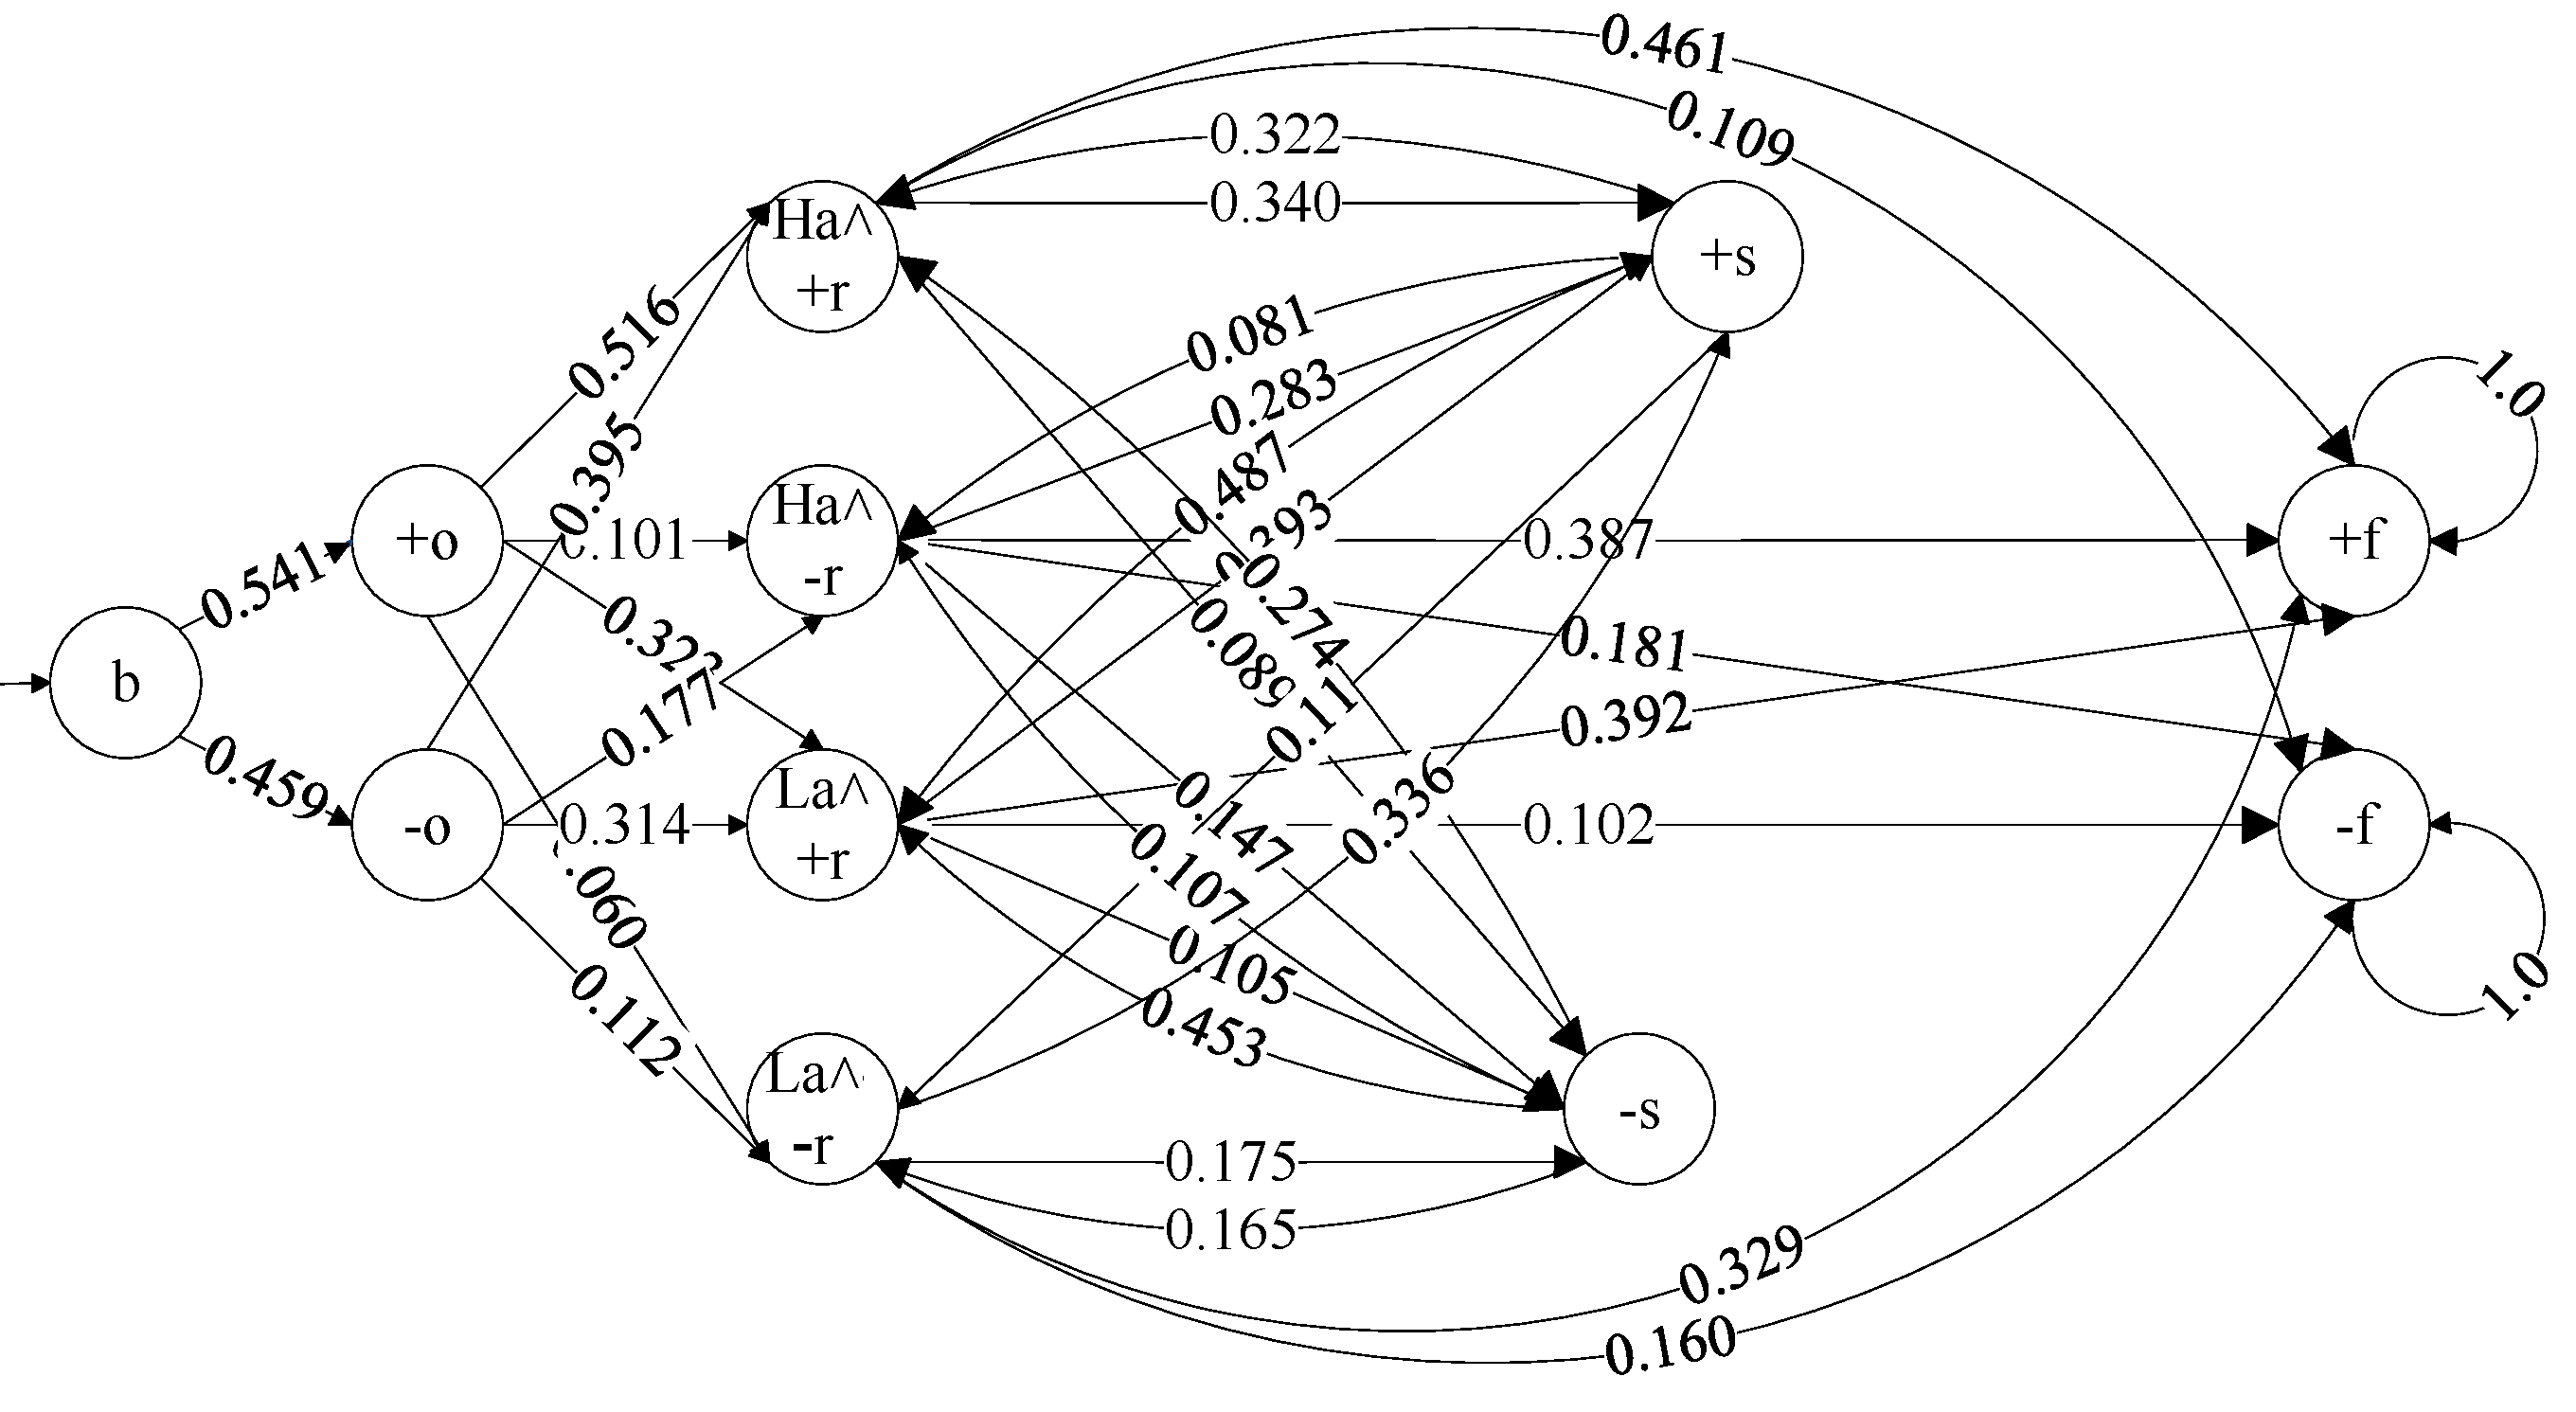
\includegraphics[width=0.99\linewidth]{Figures/model_lex.pdf}
  \caption{A probabilistic Kripke Structure modeling the sentiment of the latest self-reply using sentiment scores and lexical alignment measures (LILLA)}\label{fig:PCTL_Lex}
  \up
\end{figure}

\begin{figure}[!htb]
 \centering
  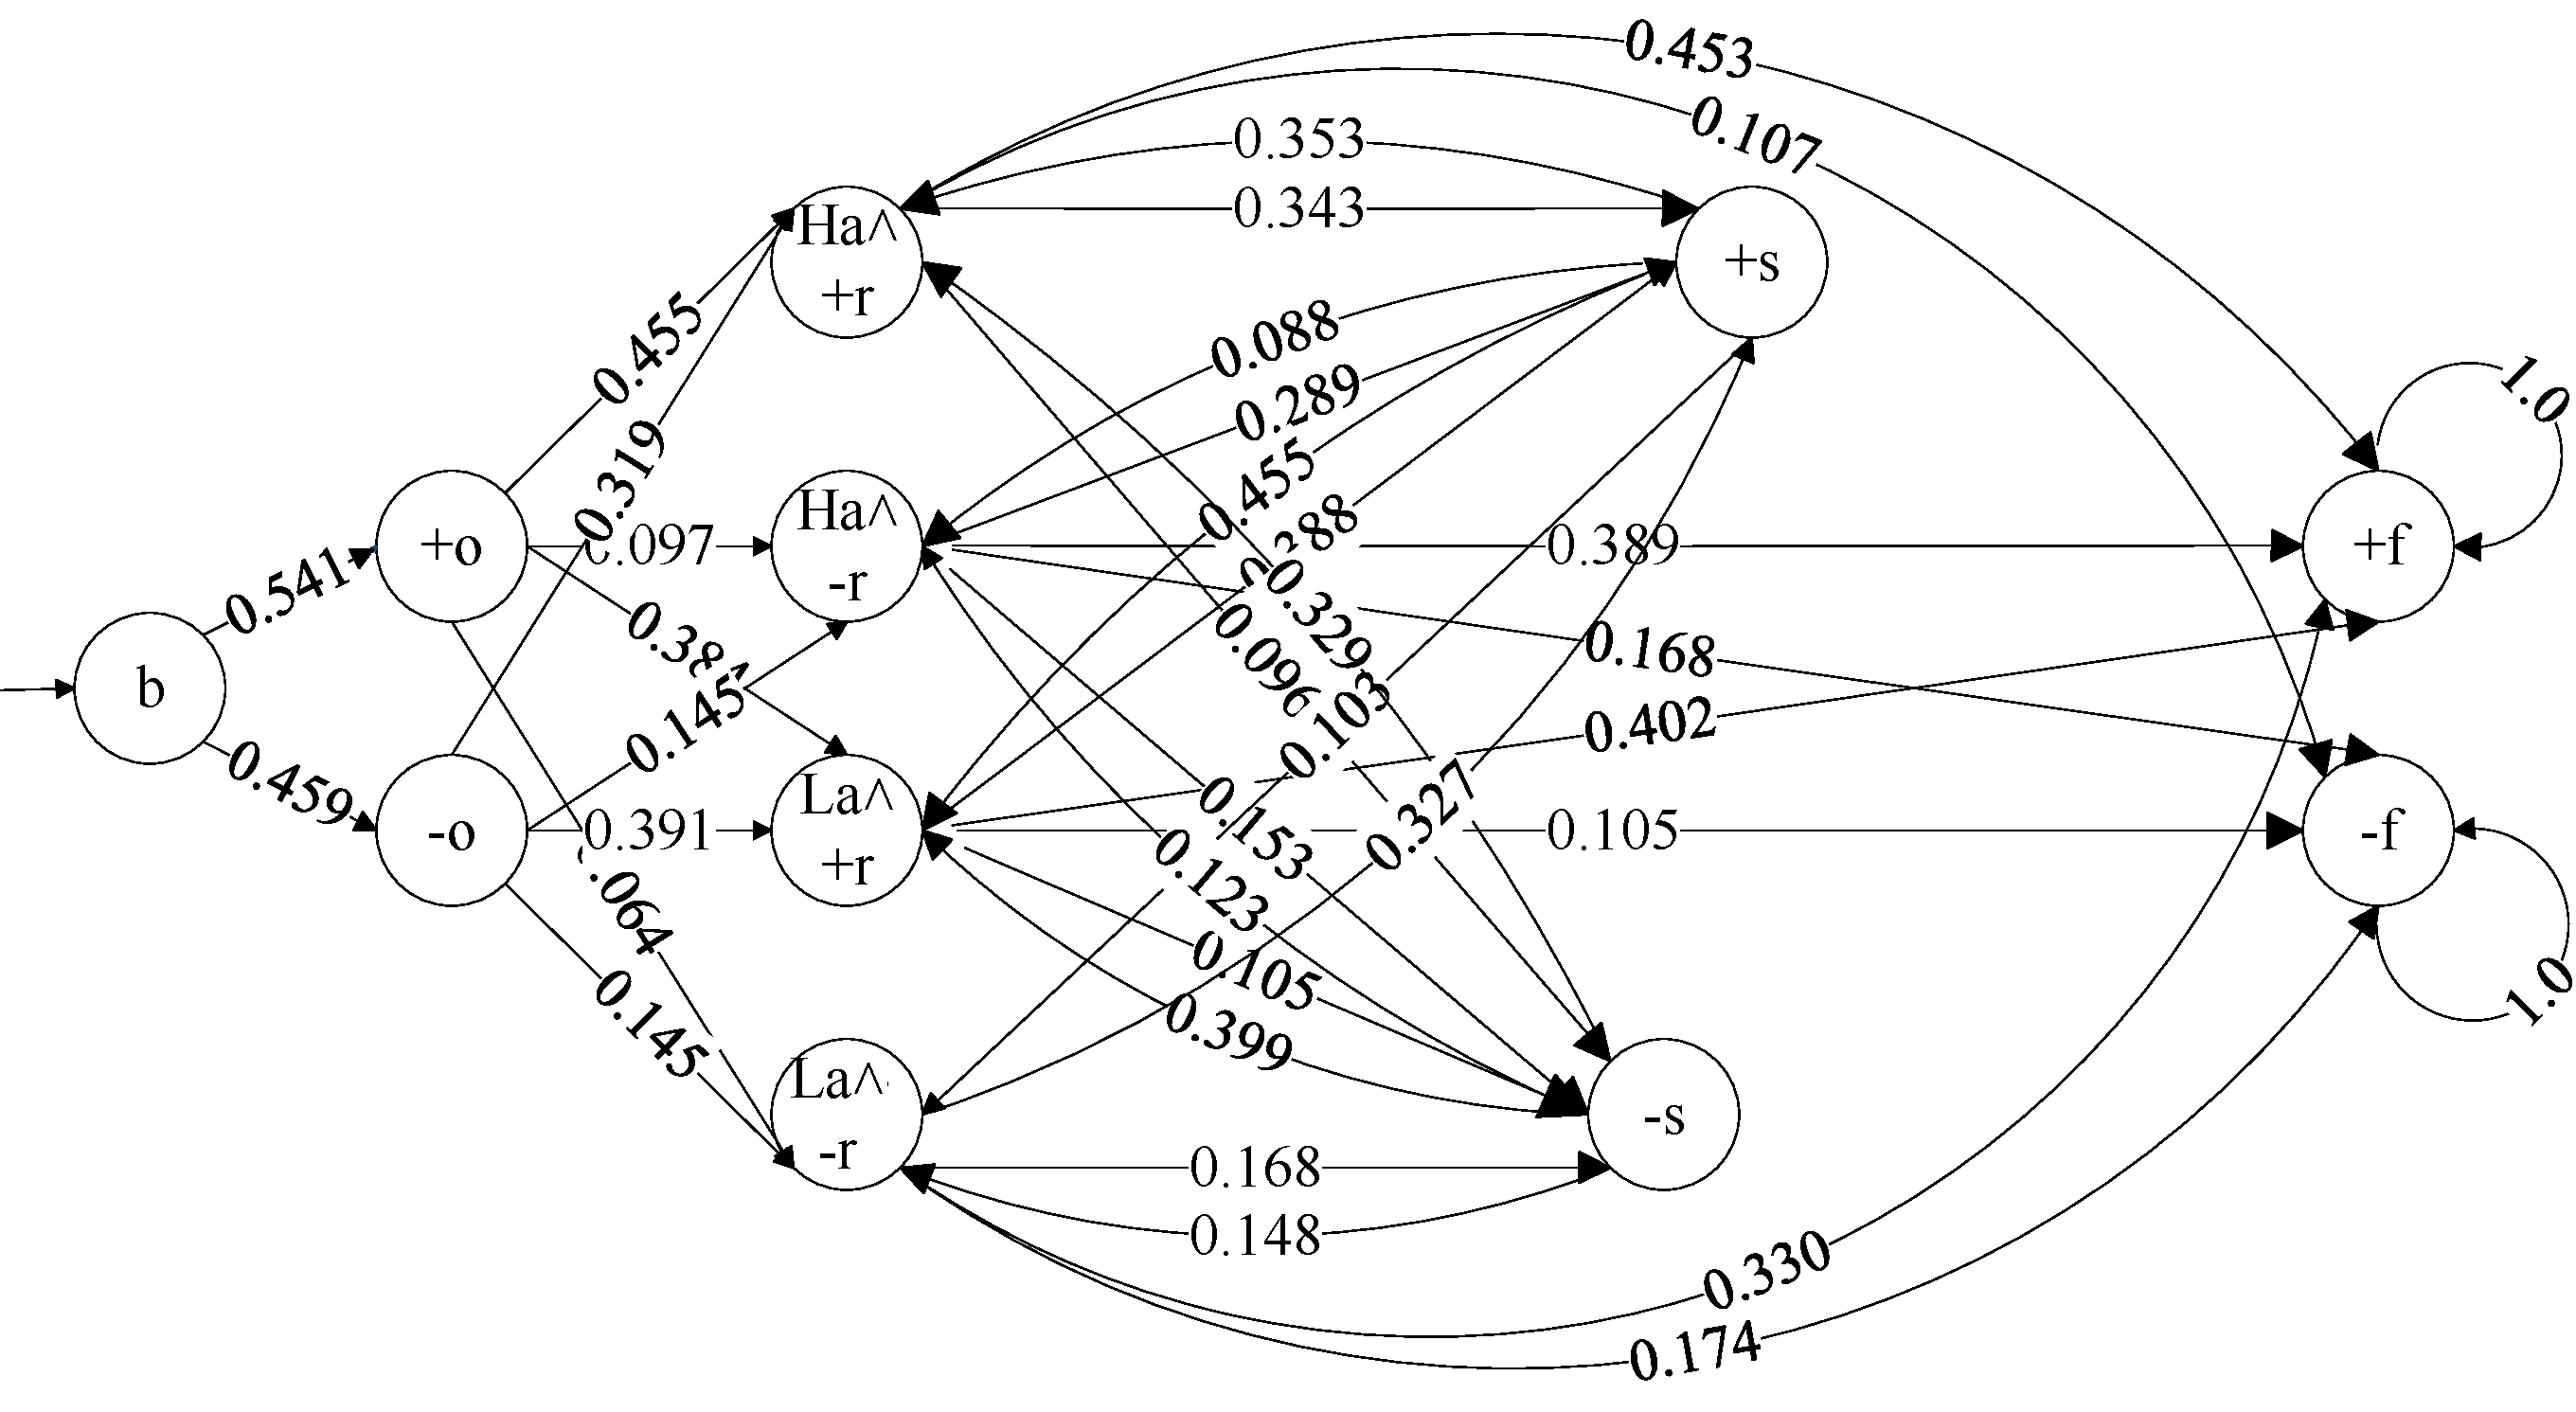
\includegraphics[width=0.99\linewidth]{Figures/model_syn.pdf}
  \caption{A probabilistic Kripke Structure modeling the sentiment of the latest self-reply using sentiment scores and syntactic alignment measures (SILLA)}\label{fig:PCTL_Syn}
  \up
\end{figure}


\subsection{Inferring Prima Facie Causes}

We explore the \emph{prima facie} causes of the latest sentiment of the thread initiator, $+f$ and $-f$, in a thread. The probabilities of $F^{\leq \infty }c$, $c\leadsto^{\geq 1,\leq \infty}e$, and $F^{\leq \infty }e$ are estimated using the method introduced by \textcite{kleinberg_uai09} with the two probabilistic Kripke structures in Figure~\ref{fig:PCTL_Lex} and~\ref{fig:PCTL_Syn}.

Suppose we want to examine whether the positive sentiment together with high lexical alignment of replies, $+A_{LEX} \wedge +r$, is a prima facie cause of the positive sentiment of the latest post from thread initiator, $+f$, in a thread. With a cause $c=+A_{LEX} \wedge +r$ and an effect $e=+f$, $c$ is a prima facie cause of $e$ if the probability of $c$ is larger than zero and the probability of $e$ conditional on $c$ is larger than the marginal probability of $e$ given the probabilistic Kripke structure in Figure~\ref{fig:PCTL_Lex}. Calculated using \textcite{hansson1994logic}, $+A_{T}\wedge+r$ is a prima facie cause of $+f$, since $+A_{T}\wedge+r\leadsto^{\geq 1,\leq \infty}+f = 0.618 $ and $b\leadsto^{\geq 1,\leq \infty}+f = 0.586$, where $b$ is the initial state in Figure~\ref{fig:PCTL_Lex} and~\ref{fig:PCTL_Syn}. Similarly, we calculate $c\leadsto^{\geq 1,\leq \infty}+f$ where $c \in \left \{+o, -o, +A_{T}\wedge+r, +A_{T}\wedge-r, -A_{T}\wedge+r, -A_{T}\wedge-r, +s, -s \right \}$. Then, $\left \{ +o, +A_{T}\wedge +r \right \}$ and $\left \{ -o, +A_{T}\wedge -r, -A_{T} \wedge -r, -s \right \}$ are prima facie causes of $+f$ and $-f$, respectively, in both lexical and syntactic probabilistic Kripke structures. Our results parallel with the results in \textcite{bui2015temporal} who state that $+r$ and $-r$ are prima facie causes of $+f$ and $-f$, respectively.


%Similarly, the negative sentiment of replies, $-r$, is a prima facie cause of the final negative sentiment of the thread initiator, $-f$.
Surprisingly, in our two models (lexical and syntactic alignment models), only $+A_T \wedge +r$ is the prima facie cause of $+f$, which indicates that linguistic alignment at both lexical and syntactic levels play an critical role in changing the sentiment of the thread initiator from negative to positive. %

% add properties

In addition to conditions of prima facie causes, a further property, \emph{complementary prima facie cause}, is inspired by the prima facie cause analysis on $+f$.
\begin{defn}
\textbf{Given $C=[c_{1}, c_{2}, \cdots, c_{n}]$ is a set of potential atomic causal factors of $e$, $\left \langle c_{1}, c_{2}, \cdots , c_{n} \right \rangle$ is a set of complementary Prima Facie Causes of $e$ if and only if: (1) $C_{cause}=c_{1} \wedge c_{2} \wedge \cdots \wedge c_{n}$ is a prima facie cause of $e$; (2) $\forall C_{i}= V_{c_{1}} \wedge V_{c_{2}} \wedge \cdots \wedge V_{c_{n}}$, $C_{i}$ is not a prima facie cause of $e$, where $V_{c_{i}} \in \left \{ c_{i}, \neg c_{i}\right \}$, and $C_{i} \neq C_{cause}$.}
\end{defn}
Intuitively, a set of potential atomic causal factors forms a set of complementary
prima facie causes of an effect iff (1) the factors together (i.e., the conjunct) forms a prima facie cause of $f$, and (2) the negation of any combination of the factors in the conjunct renders the conjunct to be {\em not} a prima facie cause of f. For example, we found that a reply posts' positive sentiment and its high lexical alignment with the thread initiating post are \emph{complementary prima facie causes} of the final positive sentiment of thread initiator, $+f$.
However, high syntactic alignment and positive sentiment of reply posts are {\em not} complementary prima facie causes, because low syntactic alignment together with positive sentiment still form a prima facie cause.


% \begin{figure}[!htb]
%  \centering
%   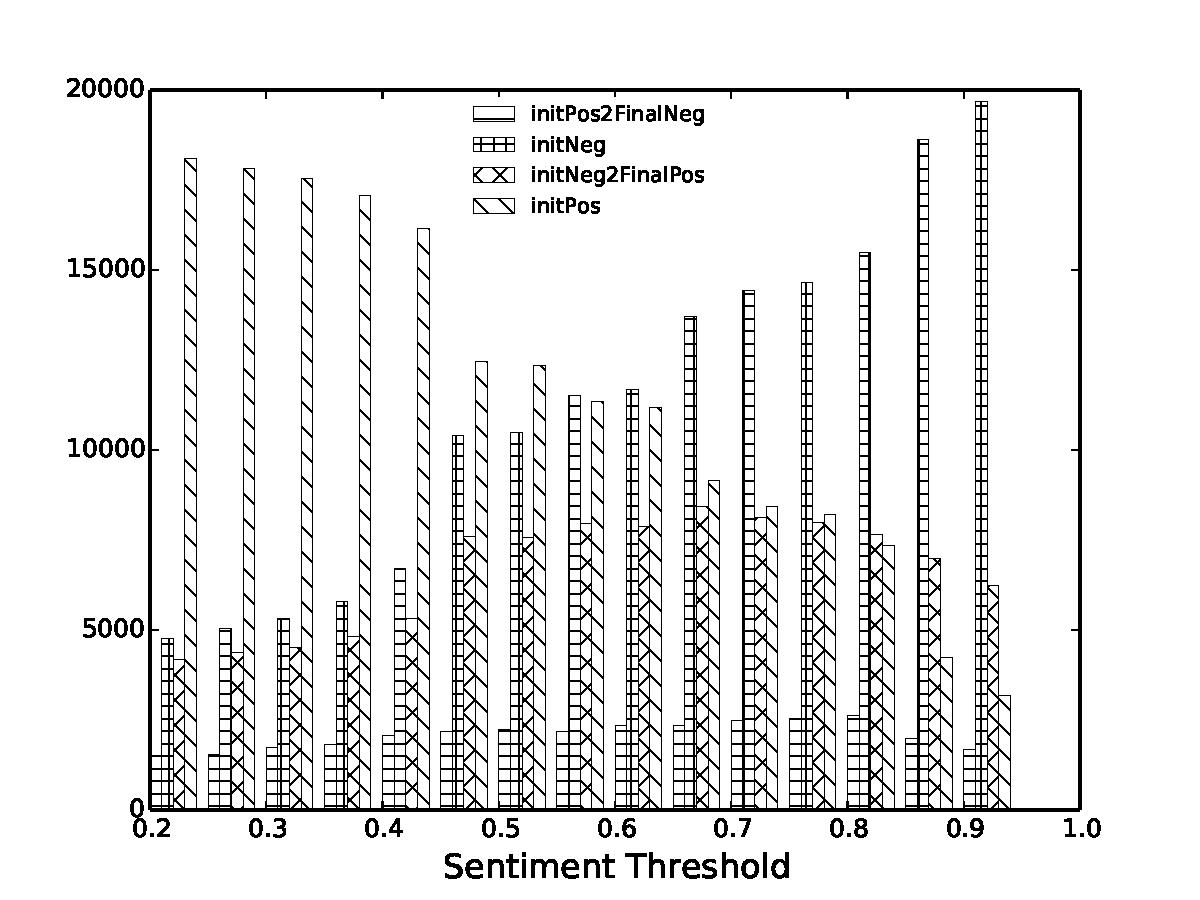
\includegraphics[width=1.0\linewidth]{barGraphs.pdf}
%   \caption{\label{fig:barSentimentTransition} Bar graphs of sentiment change on different classification theshold}
% \end{figure}

\subsection{Significance of Prima Facie Causes}

We proceed to assess the significance of the prima facie causes of $+f$ and $-f$. Table~\ref{tab:CausalSig} shows the causal significance of these prima facie causes from alignment perspectives using~\ref{def:CausalSig}.

First, we would like to caution the reader with regard to the meaning of \emph{significance}, which, in \citegen{kleinberg_uai09} framework requires an empirically estimated threshold for $\epsilon$ that serves to avoid false positive findings of significance (akin to statistical signifiance, a.k.a. reliability).  In the analysis that follows, we calculate the significance scores associated with low and high alignment (as cause), examining whether one reliably exceeds the other.

$\epsilon(+A_T \wedge +r, +f)$ appears in both lexical and syntactic alignment models. In other words, sentiment-positive replies that are either high lexical aligned or high syntactic aligned play a key role in changing the sentiment of the latest post from the thread initiator in a thread. By contrast, sentiment-positive replies that are either low lexically aligned or low syntactically aligned, are not causally significant. Hence, high alignment at both lexical and syntactic level is a meaningful predictor for the final positive sentiment change.

In addition, both $\epsilon(+A_{T} \wedge -r, -f)$ and $\epsilon(-A_{T} \wedge -r, -f)$ are causal significant in both lexical and syntactic alignment models. Specifically, $\epsilon(+A_{T}\wedge -r, -f)$ is smaller than $\epsilon(-A_{T} \wedge -r, -f)$. It suggests that replies with negative sentiment have a stronger causal significant effect in combination with low alignment score than with high alignment score, at both lexical and syntactic levels in  \citegen{kleinberg_uai09}  framework. Therefore, we conclude that the linguistic alignment of replies at both lexical and syntactic levels, together with the sentiment of the replies, causally affect the final sentiment change of the thread initiator.


\begin{table}[]
\centering
\begin{tabular}{l|l|l}
                             & Lexical & Syntactic \\ \hline
$\epsilon(+A_{T} \wedge +r, +f)$ & 0.033   & 0.030     \\ \hline
$\epsilon(+A_{T} \wedge -r, -f)$ & 0.028   & 0.020     \\ \hline
$\epsilon(-A_{T} \wedge -r, -f)$ & 0.046   & 0.051     \\ \hline
\end{tabular}
\caption{Level of Causal Significance of Alignment}
\label{tab:CausalSig}
\end{table}


\subsection{Impact of the choice of Linguistic Alignment Measures}

% Enlarge font
\begin{figure}[!htb]

\begin{subfigure}{.5\textwidth}
  \centering
  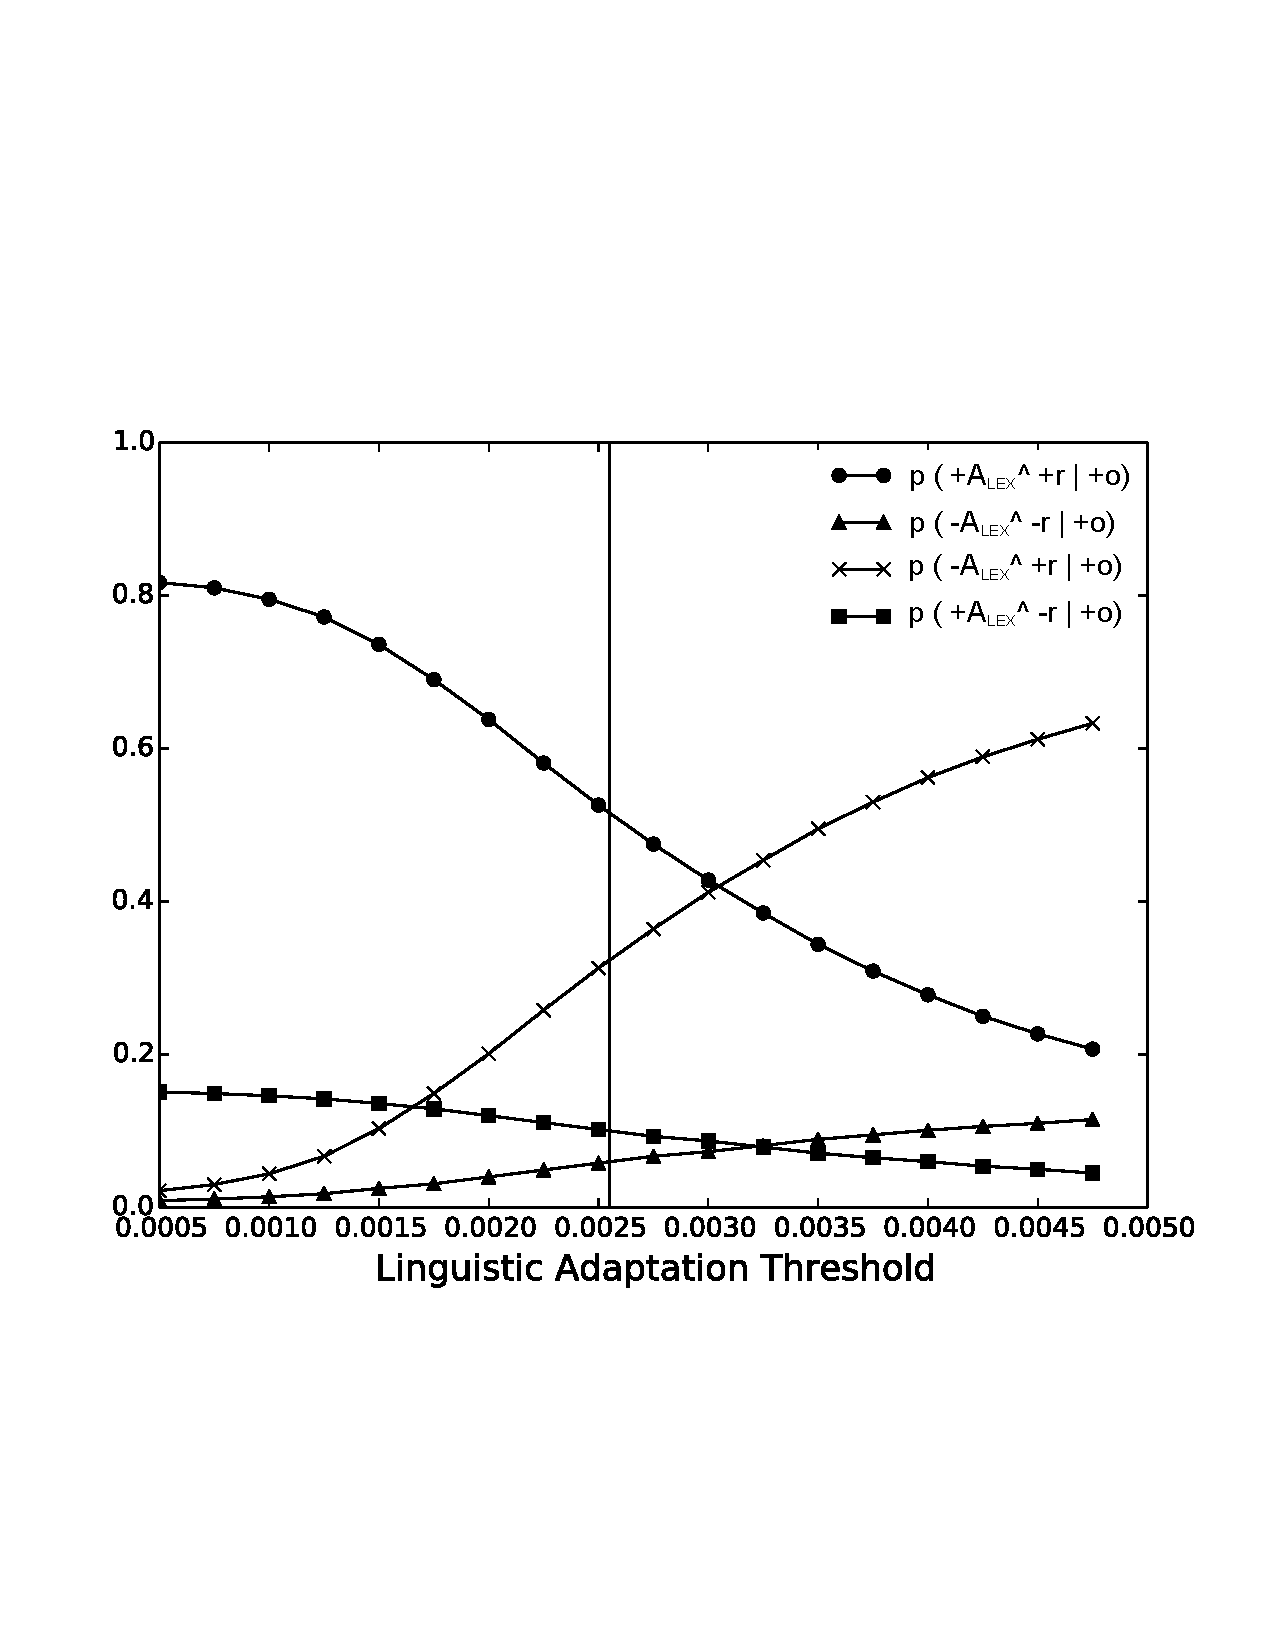
\includegraphics[width=\linewidth]{Figures/LexAposi_new_rob_New_Enlarge.pdf}
  \caption{\label{fig:ProbLexPoso}}
\end{subfigure}%
\begin{subfigure}{.5\textwidth}
  \centering
  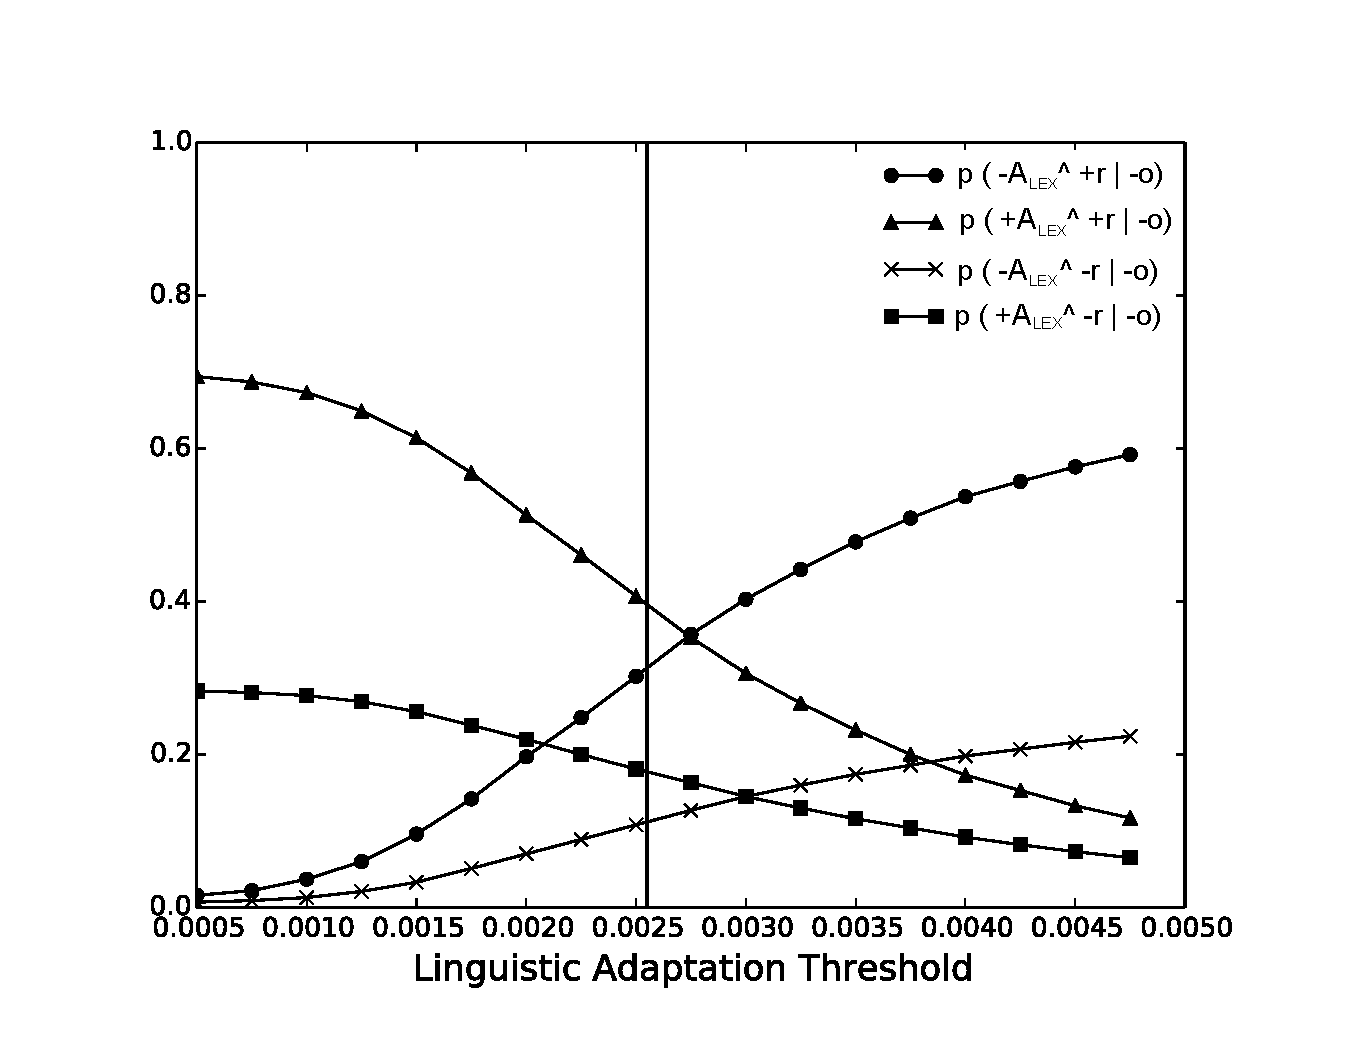
\includegraphics[width=\linewidth]{Figures/LexAnegi_new_rob_New_Enlarge.pdf}
  \caption{\label{fig:ProbLexNego}}
\end{subfigure}%
\caption{Probabilities of replies with different sentiment and lexical alignment score condition on the sentiment score of the initial post. Vertical lines indicate the thresholds we choose in each model.}
\label{fig:Probability_Change_Lex}
\up
\end{figure}

\begin{figure}[!htb]
\begin{subfigure}{.5\textwidth}
  \centering
  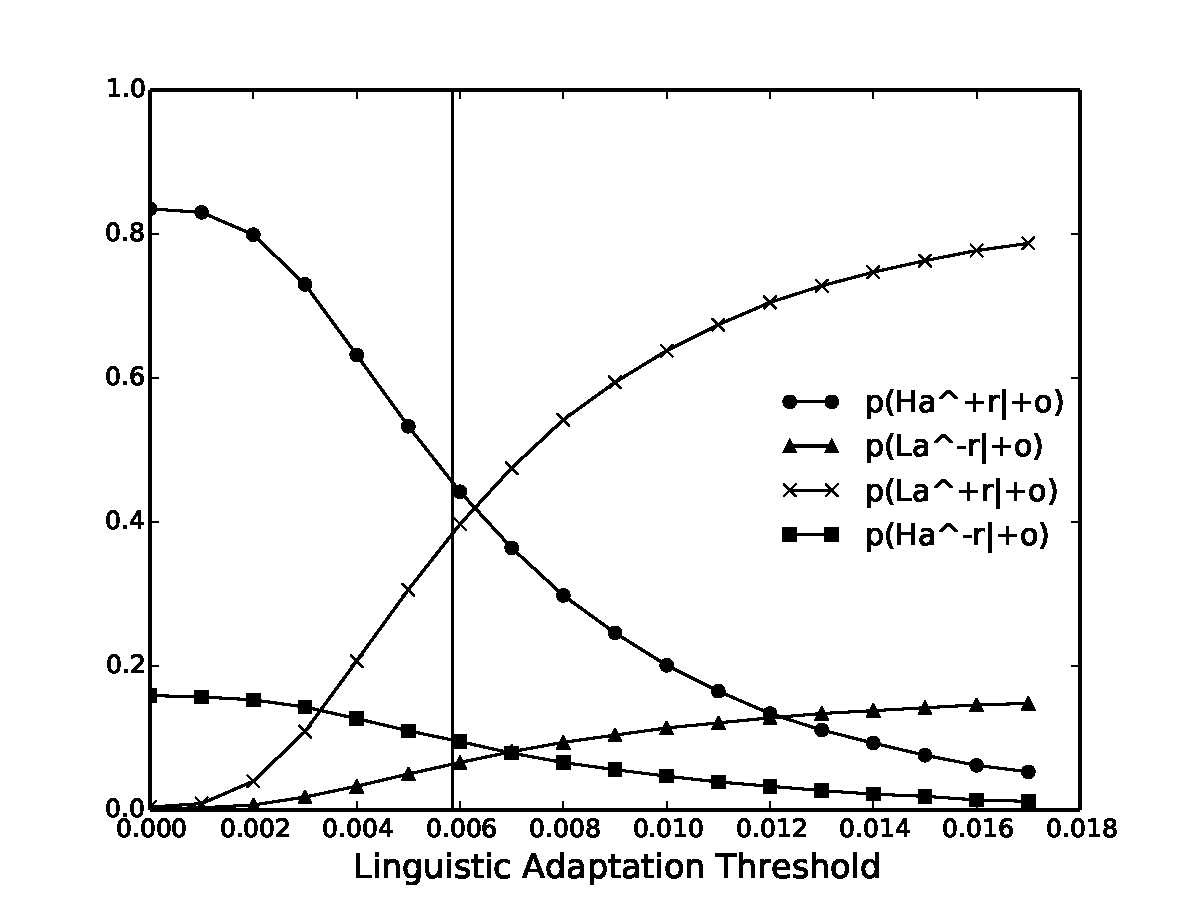
\includegraphics[width=\linewidth]{Figures/SynAposi_new_rob_New_Enlarge.pdf}
  \caption{\label{fig:ProbSynPoso}}
\end{subfigure}%
\begin{subfigure}{.5\textwidth}
  \centering
  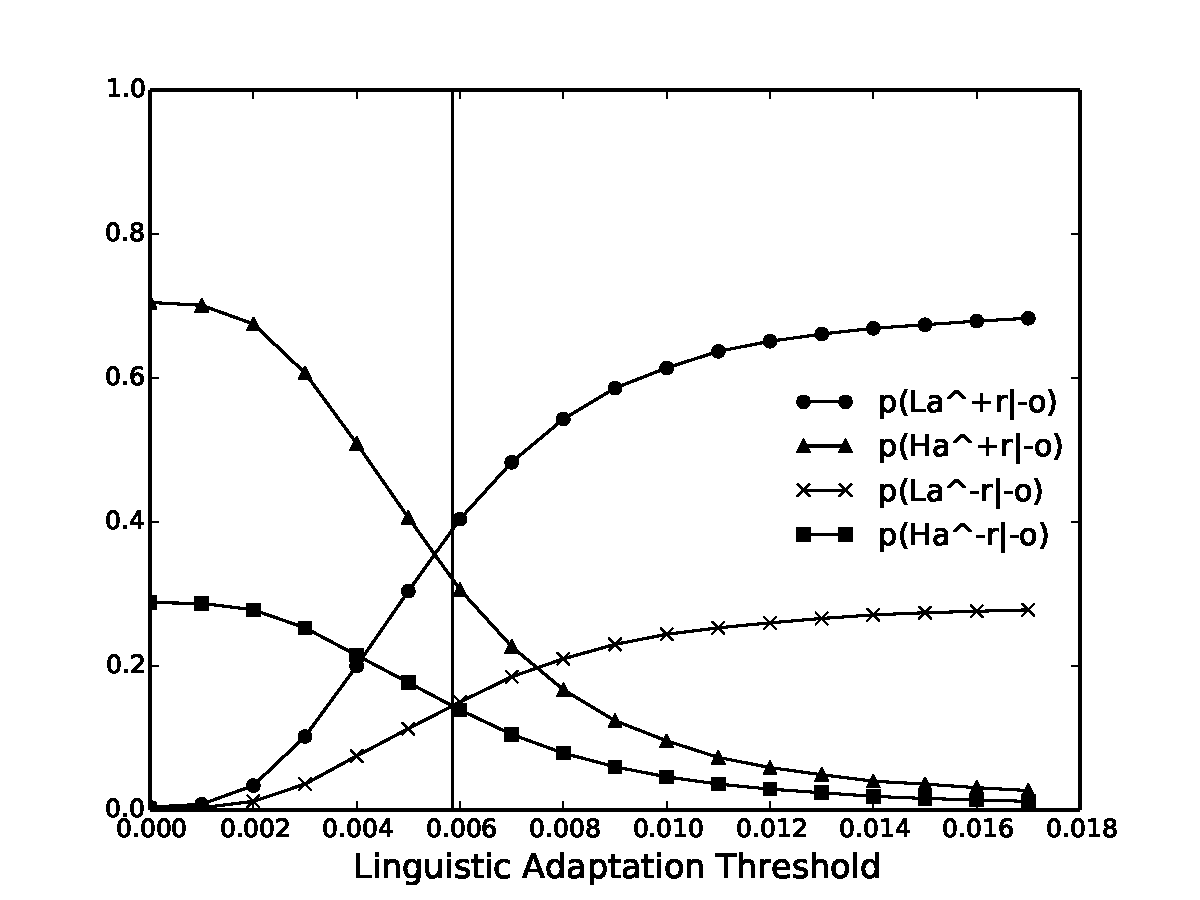
\includegraphics[width=\linewidth]{Figures/SynAnegi_new_rob_New_Enlarge.pdf}
  \caption{\label{fig:ProbSynNego}}
\end{subfigure}%
\caption{Probabilities of replies with different sentiment and syntactic alignment score condition on the sentiment score of the initial post. Vertical lines indicate the thresholds we choose in each model.}
\label{fig:Probability_Change_Syn}
\up
\end{figure}


Next, we investigate how the threshold of linguistic alignment affects the transition probabilities in our probability Kripke structures. We investigate a range of values for linguistic alignment threshold around our threshold (the median value of linguistic alignment in this dataset). The lexical alignment threshold (LILLA) changes from 0.0005 to 0.0047, and the syntactic alignment threshold (SILLA) changes from 0.000 to 0.017.


Figure~\ref{fig:ProbLexPoso} and~\ref{fig:ProbLexNego} show the probability of positive and negative replies with different levels of lexical alignment when the thread is initiated with a negative post and a positive post, respectively. Comparing the probability dynamics of replies with high or low lexical alignment, we note that the probabilities of high lexical alignment is higher than that of low lexical alignment. Members in CSN tend to align with words of the initial post, no matter the sentiment of the initial post.

Also, Figure~\ref{fig:ProbSynPoso} and~\ref{fig:ProbSynNego} show the probability of positive and negative replies with different levels of syntactic alignment when the thread is initiated with a negative post and a positive post, respectively. Unlike in the case of a probabilistic Kripke structure based on a lexical alignment model, there is less syntactic alignment on the thread initiator if the thread is initiated with a post with negative sentiment. Although lexical and syntactic alignment models show that aligned replies are causal factors of the sentiment of the last self-reply in a thread, these results show that syntactic alignment is more sensitive than lexical alignment on the threshold we choose.




\subsection{Impact of the choice of linguistic alignment thresholds}

We have shown that linguistic alignment is a potential causal factor of the sentiment of the last self-reply in a thread. Next, we explore how causal significance changes, given various lexical and syntactic alignment thresholds, on the sentiment of the last self-reply. Figure~\ref{fig:Robust_Lex} and Figure~\ref{fig:Robust_Syn} show the causal significance of prima facie causes, $-A_T \wedge +r$ and $+A_T \wedge +r$, of the effect $+f$ and $-f$ using lexical and syntactic alignment scores, respectively.

\begin{figure}[!htb]
\begin{subfigure}{.5\textwidth}
  \centering
  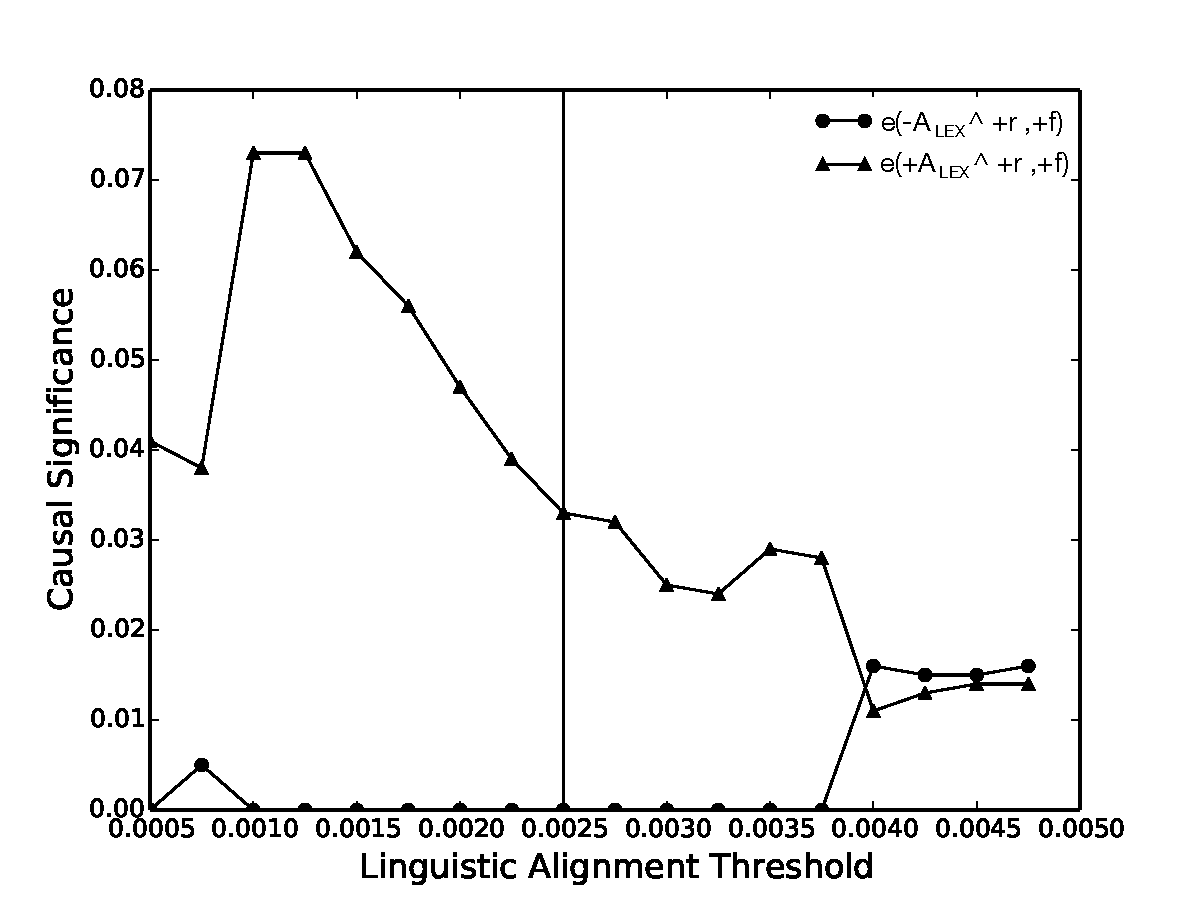
\includegraphics[width=\linewidth]{Figures/EnlargeposF05Lex20.pdf}
  \caption{\label{fig:posf05Lex}}
\end{subfigure}
\begin{subfigure}{.5\textwidth}
  \centering
  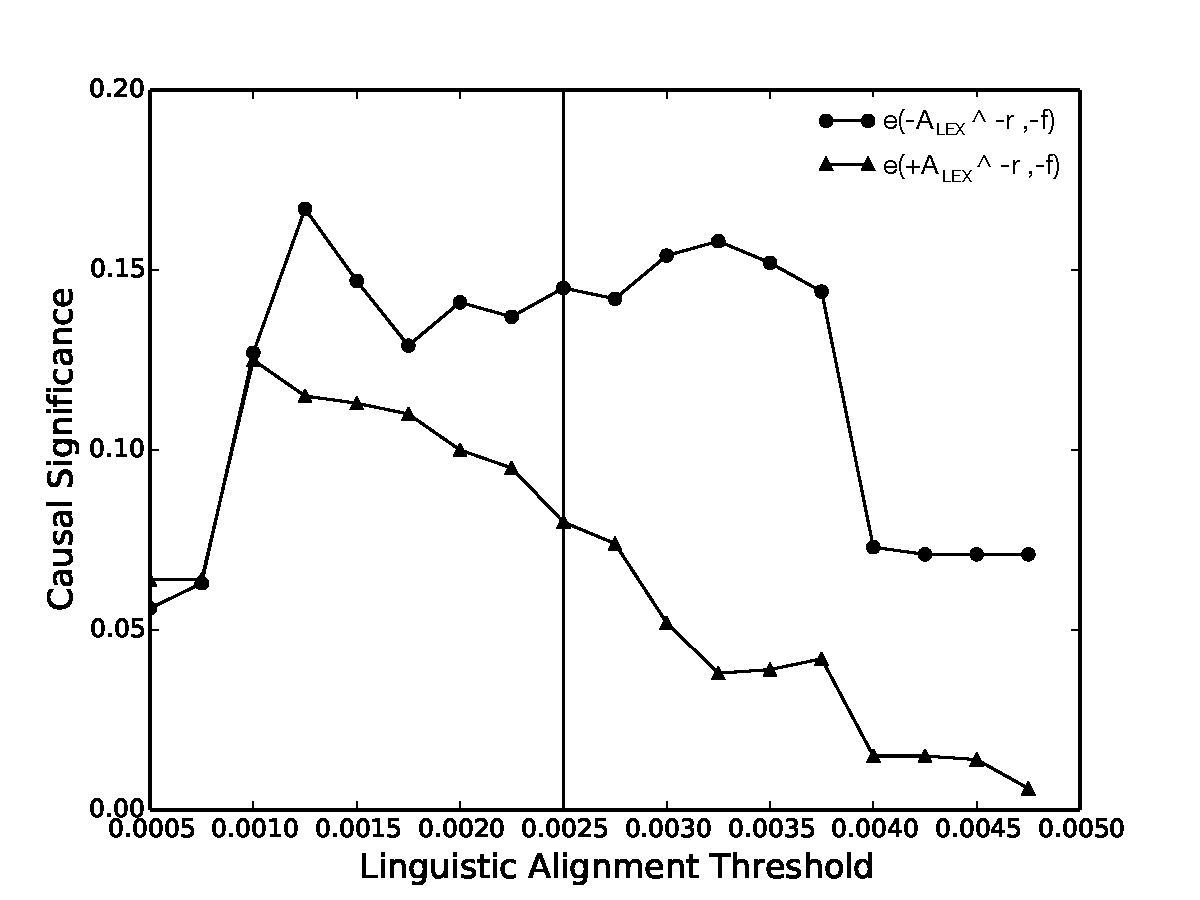
\includegraphics[width=\linewidth]{Figures/EnlargenegF05Lex20.pdf}
  \caption{\label{fig:negf05Lex}}
\end{subfigure}
\caption{Causal significance analysis on sentiment change of the thread initiator using lexical alignment and sentiment score of replies. The vertical line shows the threshold we choose.}
\label{fig:Robust_Lex}
\end{figure}

Figure~\ref{fig:posf05Lex} shows that $+A_{LEX} \wedge +r$ consistently shows up as a prima facie cause. As the threshold of lexical alignment increases, the causal significance of $+A_{LEX} \wedge +r$ drops steadily. However, $-A_{LEX} \wedge +r$ is not considered as a prima facie cause (i.e., the causal significance of $-A_{LEX} \wedge +r$ is zero). This result parallels with the result in the previous section. Therefore, we conclude that $+A_{LEX} \wedge +r$ using the lexical alignment score is a genuine cause of $+f$, but $-A_{LEX} \wedge +r$ is not. This finding indicates that having replies with high \emph{lexical alignment} is an important factor on sentiment dynamics of the thread initiator in this OHC.

Figure~\ref{fig:negf05Lex} suggests that, for lexical alignment, both $+A_{LEX} \wedge -r$ and $-A_{LEX} \wedge -r$ are prima facie causes of $-f$. However, the causal significance of $-A_{LEX} \wedge -r$ is consistently and reliably higher than that of $+A_{LEX} \wedge -r$ on $-f$ (Wilcoxon signed-rank test, $p<0.0005$) . This result indicates that messages with negative sentiment combined with lower lexical alignment likely cause the negative sentiment of thread initiator's final message in a thread. This finding parallels our causal analysis on $+f$ that messages with higher lexical alignment complemented with positive sentiment contribute on thread initiators' positive sentiment at the end of a thread. Further, the effect of $-A_{LEX} \wedge -r$ on $-f$ is larger than that of $+A_{LEX} \wedge -r$ on $-f$.

\begin{figure}[!htb]
\begin{subfigure}{.5\textwidth}
  \centering
  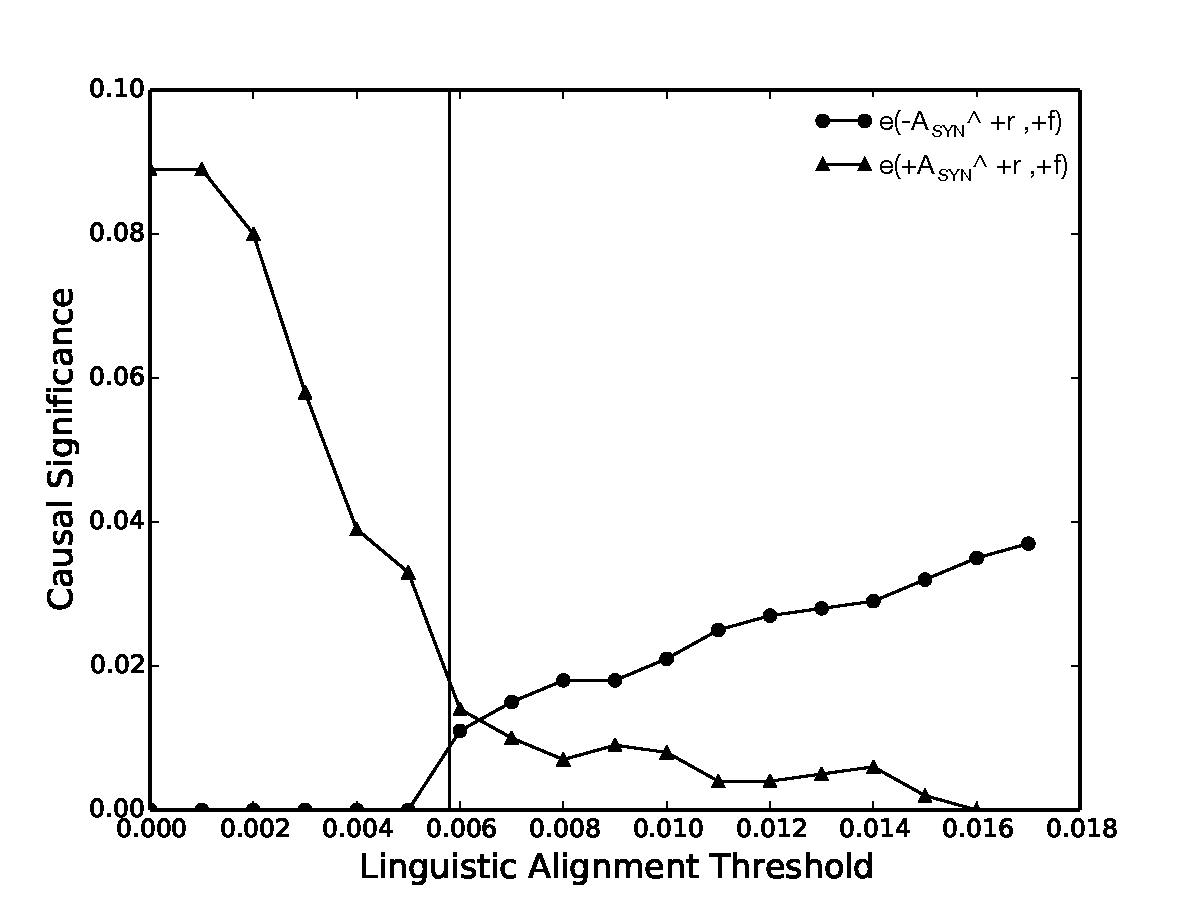
\includegraphics[width=\linewidth]{Figures/EnlargeposF05Syn_20.pdf}
  \caption{\label{fig:posf05Syn}}
\end{subfigure}
\begin{subfigure}{.5\textwidth}
  \centering
  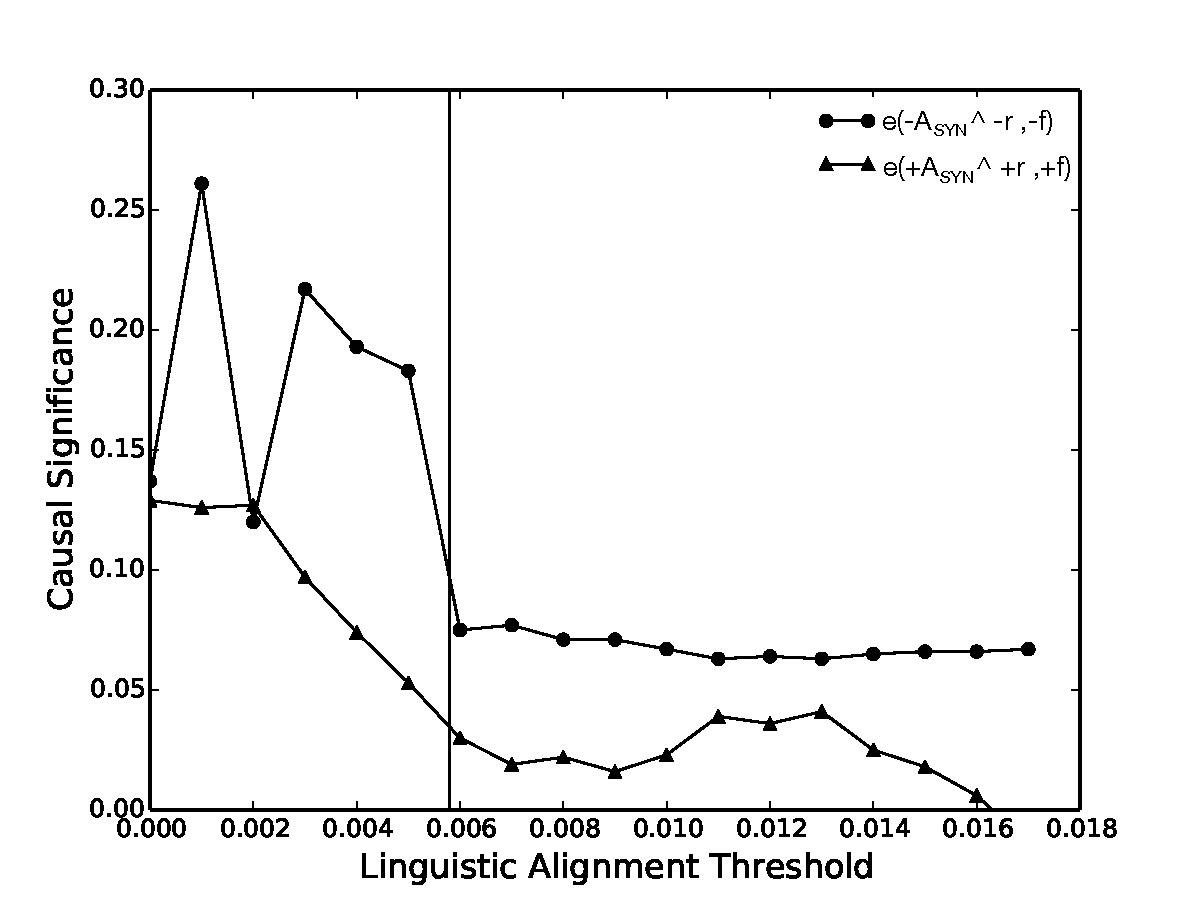
\includegraphics[width=\linewidth]{Figures/EnlargenegF05Syn_20.pdf}
  \caption{\label{fig:negf05Syn}}
\end{subfigure}
\caption{Causal significance analysis on sentiment change of the thread initiator using syntactic alignment and sentiment score of replies}
\label{fig:Robust_Syn}
\end{figure}

Further, Figure~\ref{fig:posf05Syn} shows that $+A_{SYN} \wedge +r$ consistently shows up as a prima facie cause. The causal significance of $+A_{SYN} \wedge +r$ drops substantially after increasing the threshold a little bit. However, $-A_{SYN} \wedge +r$ is considered as a prima facie cause after increasing the threshold a little bit (i.e., the causal significance of $-A_{SYN} \wedge +r$ is not zero). Therefore, we conclude that $+A_{SYN} \wedge +r$ likely causes $+f$. This finding indicates that having replies with high \emph{syntactic alignment} is not a strong factor on sentiment dynamics of the thread initiator in this OHC.

Figure~\ref{fig:negf05Syn} shows that both $+A_{SYN} \wedge -r$ and $-A_T \wedge -r$ with the syntactic alignment score are prima facie causes of $-f$. However, the causal significance of $-A_{SYN} \wedge -r$ is consistently and reliably higher than that of $+A_{SYN} \wedge -r$ on $-f$ (Wilcoxon signed-rank test, $p<0.0005$). Thus, messages with negative sentiment complemented by lower syntactic alignment likely cause a more negative sentiment in the thread initiator's final message. This finding complements the causal analysis on $+f$, which suggests that messages with higher syntactic alignment paired with positive sentiment contribute to thread initiators' positive sentiment at the end of a thread. Further, the effect of $-A_{SYN} \wedge -r$ on $-f$ is larger than that of $+A_{SYN} \wedge -r$ on $-f$.
% Is the effect larger, or do we have stronger evidence (p)?
% saying that epsilon (a p value) is higher in one
% case than another seems like a misuse of p values
% if actual effects are compared, do we have
% hypothesis tests to make sure they are different?

In summary, positive messages with high \emph{lexical} alignment are a genuine cause of the positive sentiment of the thread initiator's final message. Positive messages with high \emph{syntactic} alignment represent a weaker cause.


\subsection{Impact of accuracy of sentiment classification}

Because we use the sentiment classifier developed by \textcite{qiu2011get} for labelling posts, it is possible that the sentiment labels are incorrect. The  framework introduced in \textcite{kleinberg_uai09} can only model states which are represented accurately. Hence, we use the framework introduced in \textcite{bui2016temporal}, which relaxes this assumption. Specifically, the Bui-Yen-Honavar's temporal causal inference model incorporates the performance (Positive Predictive Value, $PPV=0.848$, Negative Predictive Value, $NPV= 0.670$) of the sentiment classifier estimating the distribution of true labels into our analysis of causal significance.
We found that in the resulting updated Kripke structure, $+A_T \wedge +r$ is a prima facie cause of $+f$, but $-A_T \wedge +r$ is not in both lexical and syntactic models. Also, both $+A_T \wedge -r$ and $-A_T \wedge -r$ are prima facie causes of $-f$. We conclude that our findings of causal significance are robust to errors in sentiment classification.


\section{Discussion}



%Understanding the benefits of participation in an OHC, such as CSN, calls for a causal account of these benefits. The online forum of cancer survivors provide a uniquely rich data source for exploring such a causal account. This paper builds on and extends the framework of \textcite{bui2016temporal} to examine the role of linguistic  alignment  between  conversation thread initiating posts and the responses in bringing about a  positive  change  in  the  sentiment  of  the  conversation thread initiator.




Two observable variables contribute to  a  positive  change  in  the  sentiment  of  the thread originator: (1) lexical  alignment  between the thread initiating post and the reply posts, and (2) a positive sentiment  of  reply  posts.  These conclusions are robust with respect to the choice of linguistic alignment thresholds and the accuracy of sentiment classification.

The method used to come to this conclusion is  an example of how the temporal-causal inference framework \parencite{bui2016temporal} can be applied in dialogue.
 We augment the representation of posts used by \textcite{bui2016temporal} to include an encoding of the lexical/syntactic alignment between the initial post of the thread and the replies to study the linguistic devices associated with positive emotional reinforcement.

These results also provide a new, interesting perspective to study the causal effect of linguistic alignment in web-based conversations as well as the impact of OHCs.


Our results lend support to a theory of alignment in dialogue that extends beyond mutual understanding.  They point to a system of dialogic conventions or signals that are used to infer agreement, emotional or otherwise, by adopting the interlocutor's lexical choices.  This does not, however, mean that speakers intentionally use them that way.  In fact, we can observe them aligning to context rather than addressee \parencite{reitter2017alignment,wang2014linguistic}, indicating an implicit effect that has its roots in memory and availability.  Yet, agreement or affect can be correlated with increased alignment \parencite{danescu2011chameleons}, and alignment can even be absent \parencite{healey2014divergence}.  The data we present suggest that alignment at the lexical level does have indeed an effect in the listener, causing sentiment change.

The data are also
compatible with a model of a language comprehension system where syntactic and lexical choices can make contributions to high-level meaning that are independent from each other.


Looking at the psychological theory of dialogue, we find an analogy in the Interactive Alignment Model (IAM) \parencite{pickering2004toward}, which proposes that alignment helps people improve mutual understanding.  For task-oriented dialogue, there is empirical evidence for this proposal \parencite{reitter2014,xu2017acl}.  Here, we find evidence for a relationship from lexical alignment to emotional alignment in the emotionally supportive dialogue.  However, rather than saying that alignment at one level leads to more alignment at another (as per the IAM), we find that poor linguistic alignment combined with negative emotions helps convey these emotions, and that good linguistic alignment combined with a positive message may help convey positive emotions.

% THE FOLLOWING DOESN"T MAKE SENSE IF -A_T & -s -> -f.

%So, what is the psychological mechanism that produces the effect we see, i.e., sentiment change that is facilitated by linguistic adaptation?  A plausible explanation starts with memory associations with emotions. As speakers use words in a context that triggers certain emotions, then these words and concepts become temporarily associated with these emotions. Later re-use of the words or concepts, whether by other discourse participants or by the target subject (the initiator of the conversation), tends to trigger the same emotions. Thus, lexical alignment can be expected to increase emotional adaptation and, thus, sentiment change.  The same cannot be said for sentence structure as a source of such emotional associations, as syntactic processes are routinized, depending on procedural skills rather than declarative (conceptual, lexical) memories.  Routines are fast, and they are not a source of associative cues for memories or emotions.  Only rare syntactic constructions might be more directly represented in lexical memory, and only these would trigger associated memories.

%\subsection{Summary}

%{\bf to do (DR):  revise w respect to the dialogue\&discourse journal}


\section{Conclusions}

This paper applies a graph-based causal modeling approach to a psycholinguistic question in dialog.  If we were to sum up and compare the approach, we would begin with a set of time-stamped events observed in large-scale data.  By imposing simple contraints such as that causes must precede effects, and that causes must increase the probability of an effect occurring, we can identify \emph{prima facie} causes in a graph model.  Then, an inference procedure can identify the quality of evidence available for specific causes, allowing us to do hypothesis-driven comparison.

Comparing to the now widely used linear mixed effects modeling, we observe that both methods use a form of model selection to reduce a set of potential effects to one that describes the data but also generalizes well -- based on the quality of evidence.  Temporal-causal inference provides a powerful way to take the longitudinal nature of language data into account, without the need for explicitly coming up with hypotheses about individual causal relationships between events (as in \emph{Granger causality}).  The result is an intuitive graph model in which the relative strength of evidence for causal relationships can be shown.

We have applied this concept to a pertinent question in dialogue research: do lexical and syntactic alignment support speakers in effectively conveying messages of positive and negative emotions?  The causal structure as per the data from our online health community suggests that \emph{yes}, they can, particularly for the case of lexical alignment.  However, lexical and emotional alignment do not simply form a basic cascade, with lexical alignment supporting emotional adoption of the message.  Instead, strong lexical alignment can support positive emotions, while weak lexical alignment increases the efficacy of conveying negative emotions.

The graph-based model we use is descriptive and proposes causal relationships.  Yet, the study remains observational.  For this reason, we think that a manipulative experiment is called for to examine whether people use alignment as a communicative device as suggested here, or whether it is just part of a cascade of alignment effects (as previously thought).





%\subsection{Future Work}
%Some promising directions for future work include: exploring the causal effects of (explicit as well as implicit) topics on sentiment dynamics; extending the framework to handle unobserved variables; and scaling up temporal causality analysis to very large state spaces.

\section*{Acknowledgements}
This work was supported by a collaborative agreement with
American Cancer Society, which made the data of CSN available for this Research. D.R. acknowledges funding from the National Science Foundation (IIS-1459300). The authors would like to thank K. Portier, G. Greer of the
American Cancer Society, current and former members of the Cancer
Informatics Initiative at Penn State for useful discussions and comments.



\printbibliography
\end{document}
